\documentclass[a4]{article}
\usepackage[utf8]{inputenc}
\usepackage{verbatim}
\usepackage{graphicx}
\usepackage{algorithm}
\usepackage{clrscode}
\usepackage[draft]{fixme}
\usepackage{amsmath}
\usepackage{amsthm}
\usepackage{textcomp}
\usepackage{enumerate}

\usepackage{prettyref}
\newcommand{\sectionname}{Section}
% \renewcommand{\figurename}{Figure}
\newcommand*{\pref}{\prettyref}
% Adds varioref to the prettyrefs.
% Replacing vref with ref to avoid page numbers
\newrefformat{cha}{\chaptername~\ref{#1}}
\newrefformat{sec}{\sectionname~\ref{#1}}
\newrefformat{fig}{\figurename~\ref{#1}}
\newrefformat{eq}{\equationname~\ref{#1}}
\newrefformat{tab}{\tablename~\ref{#1}}
\newrefformat{app}{\appendixname~\ref{#1}}
\newrefformat{alg}{Algorithm~\ref{#1}}

\title{Algorithms for Longest Common Extensions} 

\author{Jesper Kristensen, s062397}

\newtheorem{theorem}{Theorem}
\newtheorem{lemma}{Lemma}
\newtheorem{corollary}{Corollary}

% http://texblog.net/latex/layout/page/2/
\fontdimen2\font=0.25em% interword space
\fontdimen3\font=1em% interword stretch
\fontdimen4\font=0.10em% interword shrink

\begin{document}

\newif\ifarticle
\newif\ifreport

\reporttrue

\maketitle

\newcommand{\sortt}{\textit{sort}(n,\sigma)}
\newcommand{\LCE}{\textit{LCE}}
\newcommand{\NCA}{\textit{NCA}}
\newcommand{\RMQ}{\textit{RMQ}}
\newcommand{\SA}{\textit{SA}}
\newcommand{\SAinv}{\textit{SA}^{-1}} % math
\newcommand{\SAi}{SA$^{-1}$} % no math
\newcommand{\LCP}{\textit{LCP}}
\newcommand{\LA}{\textit{LA}}
\newcommand{\suff}{\textit{suff}}
\newcommand{\logceil}{\lceil\log n\rceil}
\newcommand{\fprint}[1][k]{\ensuremath{\proc{Fingerprint}_{#1}}}
\newcommand{\fprintk}{\fprint[k]}
\newcommand{\RMQpq}[2]{RMQ\textless$#1$, $#2$\textgreater}
\newcommand{\RMQn}{\RMQpq{1}{n}}
\newcommand{\RMQq}{\RMQpq{n}{1}}
\newcommand{\RMQlog}{\RMQpq{n}{\log n}}

\hyphenation{Di-rect-Comp Di-rect-Look-up Di-rect-Comp-Look-up Fin-ger-print}

\tableofcontents

\vspace{1cm}
% stuff on toc page

\newpage

%%%%%%%%%%%%%%%%%%%%%%%%%%%%%%%%%%%%%%%%%%%%%%%%%%%%%%%%%%%%%%%%%%%%%%%%%%%%%%%
%%%%%%%%%%%%%%%%%%%%%%%%%%%%%%%%%%%%%%%%%%%%%%%%%%%%%%%%%%%%%%%%%%%%%%%%%%%%%%%
\section{Introduction\label{sec:intro}}

The Longest Common Extension problem can be used in many algorithms for solving other algorithmic problems, e.g.\ the Landau-Vishkin algorithm for approximate string searching~\cite{approx-search}. Optimal solutions exists for the problem, with constant query time and linear space. These theoretically optimal solutions are however not the best in practice, since they have large constant factors for both time and space usage. In average cases, a much simpler solution with worst case linear time, average case constant time, and no preprocessing has significantly better practical performance. This algorithm is ideal when only average case performance is relevant. In situations where we need both average case and worst case performance to be good, none of the existing solutions are ideal.

We have found two new algorithms. They both have better than linear worst case query times, and achieves significantly better average case practical query times compared to the theoretically best algorithms. The best of these two uses string fingerprinting to achieve a time/space-tradeoff with $O(k\cdot n^{1/k})$ worst case query time, constant average case query time, and $O(kn)$ space for $k$ between one and $\log n$.

In \pref{sec:algorithms} we theoretically describe and analyze the LCE algorithms introduced here in \pref{sec:intro}, and in \pref{sec:results} we analyze results from practical C++ implementations of these algorithms.

We also look at how to apply the LCE problem to Ziv-Lempel compressed strings, such that we can answer LCE queries fast while only using space, which is a function of the compressed size of the string. In \pref{sec:lz-compress} we describe LZ compression, and how we can convert the simple linear time LCE algorithm to work on compressed strings with space linear to the size of the compressed string, worst case query time linear to the size of the uncompressed string, and average case query time $O(\log\log N)$. In \pref{sec:tree-lce} we look at how we can use the tree structure of LZ compression to get better query times on compressed strings.

%%%%%%%%%%%%%%%%%%%%%%%%%%%%%%%%%%%%%%%%%%%%%%%%%%%%%%%%%%%%%%%%%%%%%%%%%%%%%%%
\subsection{The LCE Problem}

Given a string $s$ of length $n$ and a pair of indexes $1\leq i\leq n$ and $1\leq j\leq n$, the Longest Common Extension of $i$ and $j$ on $s$, $\LCE_s(i,j)$, is the length of the longest common prefix of $\suff_i$ and $\suff_j$. If for example $s = abbababba$, $i = 4$ and $j=6$, then $\suff_4 = ababba$ and $\suff_6 = abba$. The longest common prefix of these two suffixes is $ab$, which has length $2$, and therefore we have $\LCE_s(4,6) = 2$.

The LCE problem is to preprocess a string in order to allow for a large number of LCE queries on different pairs $(i,j)$, such that the queries are efficient.

Given a string length $n$ and an alphabet size $\sigma$, we define average case query time as the average of query times over all $\sigma^n\cdot n^2$ combinations of strings and query inputs.

%%%%%%%%%%%%%%%%%%%%%%%%%%%%%%%%%%%%%%%%%%%%%%%%%%%%%%%%%%%%%%%%%%%%%%%%%%%%%%%
\subsection{Existing Results\label{sec:existing-results}}

One way of solving the LCE problem without any preprocessing uses $O(|\LCE(i,j)|)$ query time. We call this algorithm \proc{DirectComp}. For a query $\LCE(i,j)$, the algorithm compares $s[i]$ with $s[j]$, then $s[i+1]$ with $s[j+1]$ and so on, until the two characters differ, or the end of the string is reached. The worst case query time is $O(n)$ on a string of length $n$, and the average case query time is $O(1)$, because the average case LCE value over all possible inputs of a given string of length $n$ and alphabet size $\sigma$ is $O(1/(\sigma-1))=O(1)$~\cite{ilie-navarro-tinta}.

The LCE problem can be solved optimally with $O(1)$ worst case query time, using $O(n)$ space and $O(\sortt)$ preprocessing time. Two different ways of doing this exists.

One method, which we call \proc{SuffixNca}, uses constant time Nearest Common Ancestor queries on a suffix tree. The LCE of two indexes $i$ and $j$ is defined as the length of the longest common prefix of $\suff_i$ and $\suff_j$. In a suffix tree, the path from the root to $L_i$ has label $\suff_i$ (likewise for $j$), and no two child edge labels of the same node will have the same first character. The longest common prefix of the two suffixes will therefore be the path label from the root to the nearest common ancestor of $L_i$ and $L_j$. This gives $\LCE_s(i,j) = D[\NCA_\mathcal{T}(L_i,L_j)]$.

The other method, which we call \proc{LcpRmq}, uses constant time Range Minimum Queries on a Longest Common Prefix array. The LCP array contains the length of the longest common prefixes of each pair of neighbor suffixes in SA. The length of the longest common prefix of two arbitrary suffixes in SA can be found as the minimum of all LCP values of neighbor suffixes between the two desired suffixes, because SA lists the suffixes in lexicographical ordering, i.e. $\LCE(i,j)=\LCP[\RMQ_{\LCP}(\SAinv[i] + 1, \SAinv[j])]$, where $\SAinv[i] < \SAinv[j]$. % An example is shown in \pref{fig:sa+lcp+min}.

%%%%%%%%%%%%%%%%%%%%%%%%%%%%%%%%%%%%%%%%%%%%%%%%%%%%%%%%%%%%%%%%%%%%%%%%%%%%%%%
\subsubsection{Existing Practical Results}

Ilie~et~al.~\cite{ilie-navarro-tinta} have looked at a number of real world texts as well as texts of randomly generated characters, and found that all the texts they examined each has an average LCE of at most one, over all $n^2$ input pairs. Therefore it is interesting to have LCE algorithms, which perform good on average when the LCE value is small.

Both \proc{SuffixNca} and \proc{LcpRmq} have the same asymptotic space and times. In practice, \proc{LcpRmq} is the best of the two~\cite{ilie-navarro-tinta}. The constant factor for average case query time of \proc{DirectComp} is much smaller than the constant factor for query time of \proc{LcpRmq}, thus \proc{DirectComp} is better in practice on average case inputs than the theoretically best \proc{LcpRmq}.

\ifreport
%%%%%%%%%%%%%%%%%%%%%%%%%%%%%%%%%%%%%%%%%%%%%%%%%%%%%%%%%%%%%%%%%%%%%%%%%%%%%%%
\subsection{Our Fingerprinting Algorithm}
\fi % report
\ifarticle
%%%%%%%%%%%%%%%%%%%%%%%%%%%%%%%%%%%%%%%%%%%%%%%%%%%%%%%%%%%%%%%%%%%%%%%%%%%%%%%
\subsection{Our Results}
\fi % article

We present a new LCE algorithm based on string fingerprinting. We call our algorithm \fprintk, where $k$ is a parameter $1\leq k\leq\logceil$, which describes the number of levels used\footnote{All logarithms are base two.}.

\begin{theorem}
For a string $s$ of length $n$ and alphabet size $\sigma$, the \fprintk\ algorithm, where $k$ is a parameter $1 \leq k \leq \logceil$, can solve the LCE problem in $O(k\cdot n^{1/k})$ worst case query time and $O(1)$ average case query time using $O(k\cdot n)$ space and $O(\sortt + k\cdot n)$ preprocessing time.
\end{theorem}

The exact worst case performance of our solution depends on the amount of space you are willing to use.

\begin{corollary}
\fprint[1] is equivalent to \proc{DirectComp} with $O(n)$ space and $O(n)$ query time.
\end{corollary}

\begin{corollary}
\fprint[2] has $O(n)$ space and $O(\sqrt n)$ query time. It has two levels, where one uses a table of fingerprints and the other uses the original string.
\end{corollary}

\begin{corollary}
\fprint[\logceil] has $O(n\cdot\log n)$ space and $O(\log n)$ query time. The data structure is equivalent to the one generated by Karp-Miller-Rosenberg~\cite{karp-miller-rosenberg}, and a query only needs to do one comparison at each level.
\end{corollary}

To preprocess the $O(k\cdot n)$ fingerprints used by our algorithm, we can use Karp-Miller-Rosenberg~\cite{karp-miller-rosenberg}, which takes $O(n\log n)$ time. For $k=o(\log n)$, we can speed up preprocessing to $O(\sortt + k\cdot n)$ by using the Suffix Array and Longest Common Prefix array.

\begin{figure}[tp]
    \begin{center}
        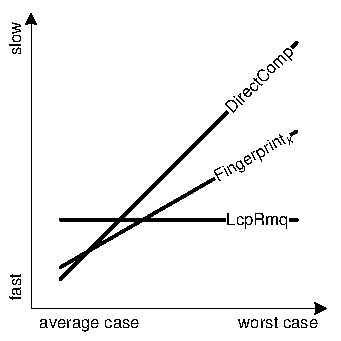
\includegraphics[width=0.5\textwidth,page=1]{wc-avg.pdf}
    \end{center}
    \caption{\label{fig:wc-avg}Graphical comparison of query times for different LCE algorithms.}
\end{figure}

Existing state of the art solutions are either good in worst case, while poor in average case (\proc{LcpRmq}), or good in average case while poor in worst case (\proc{DirectComp}). Our \fprintk\ solution targets a worst case vs. average case query time tradeoff between these two extremes. \pref{fig:wc-avg} illustrates the relative query time performances of these solutions. Our solution is almost as fast as \proc{DirectComp} on an average case input, and it is a lot faster than \proc{DirectComp} on a worst case input. Compared to \proc{LcpRmq}, our solution has a significantly better performance on an average case input, but its worst case performance is not as good as that of \proc{LcpRmq}. The space usage for \proc{LcpRmq} and \fprintk\ are approximately the same when $k=6$.

Our algorithm is fairly simple. Though it is slightly more complicated than \proc{DirectComp}, it does not use any of the advanced algorithmic techniques required by \proc{LcpRmq} and \proc{SuffixNca}.

\ifreport

%%%%%%%%%%%%%%%%%%%%%%%%%%%%%%%%%%%%%%%%%%%%%%%%%%%%%%%%%%%%%%%%%%%%%%%%%%%%%%%
\subsection{Our Table Lookup Algorithm}

We also present another new LCE algorithm, which we call \proc{DirectCompLookup}.

\begin{theorem}
For a string $s$ of length $n$, the \proc{DirectCompLookup} algorithm can solve the LCE problem in $O(t)$ worst case query time and $O(1)$ average case query time using $O(n^2/t)$ space and $O(n^2)$ preprocessing time, where $t$ is a parameter $1 \leq t \leq n$.
\end{theorem}

The algorithm stores LCE values for some of the $n^2$ possible query inputs on a given string. It uses \proc{DirectComp} to move towards one of these stored values, and stops when it reaches one. The \proc{DirectCompLookup} algorithm is very simple, but the tradeoff between worst case query time and space is not very favorable, and preprocessing the data structure takes $O(n^2)$ time unless we use another LCE algorithm in the preprocessing.

\fi % report

%%%%%%%%%%%%%%%%%%%%%%%%%%%%%%%%%%%%%%%%%%%%%%%%%%%%%%%%%%%%%%%%%%%%%%%%%%%%%%%
%%%%%%%%%%%%%%%%%%%%%%%%%%%%%%%%%%%%%%%%%%%%%%%%%%%%%%%%%%%%%%%%%%%%%%%%%%%%%%%
\section{Preliminaries}

\paragraph{String notation.} Let $s$ be a string of length $n$. Then $s[i]$ is the $i$'th character of $s$, and $s[i\twodots j]$ is a substring of $s$ containing characters $s[i]$ to $s[j]$, both inclusive. That is, $s[1]$ is the first character of $s$, $s[n]$ is the last character, and $s[1\twodots n]$ is the entire string. The suffix of $s$ starting at index $i$ is written $\suff_i = s[i\twodots n]$.

\paragraph{Tree notation.}
The ancestors of a node $u$ is $u$ itself as well as any node, which is a parent of an ancestor of $u$. The depth of a node $u$ is one greater than the depth of $u$'s parent, and the depth of the root is zero. A path in a tree begins at node $u$ and ends at node $v$, where $u$ is an ancestor of $v$.

\paragraph{Sorting complexity.} The time it takes to sort $n$ numbers of $\sigma$ distinct values is written as $\sortt$.

\paragraph{Suffix tree.} A suffix tree $\mathcal{T}$ encodes all suffixes of a string $s$ of length $n$ with alphabet $\sigma$. The tree has $n$ leaves named $L_1$ to $L_n$, one for each suffix of $s$. Each edge is labeled with a substring of $s$, such that for any $1\leq i\leq n$, the concatenation of labels on edges on the path from the root to $L_i$ gives $\suff_i$. Any internal node must have more than one child, and the labels of two child edges must not share the same first character. The string depth $D[v]$ of a node $v$ is the length of the string formed when concatenating the edge labels on the path from the root to $v$.
The tree uses $O(n)$ space, and building it takes $O(\sortt)$ time~\cite{sort-complexity}.

\ifreport

There are $n$ leaves in a suffix tree, and since each internal node has at least two children, the tree has less than $2n$ nodes. Each edge uses $O(1)$ space, as the label is a substring of $s$ and it can therefore be represented by two indexes of $s$. The suffix tree therefore takes $O(n)$ space.

\fi % report

\paragraph{SA and LCP.} For a string $s$ of length $n$ with alphabet $\sigma$, the Suffix Array, \SA, is an array of length $n$, which encodes the lexicographical ordering of all suffixes of $s$. The lexicographically smallest suffix is $\suff_{\SA[1]}$, the lexicographically largest suffix is $\suff_{\SA[n]}$, and the lexicographically $i$'th smallest suffix is $\suff_{\SA[i]}$. The inverse Suffix Array, \SAi, describes where a given suffix is in the lexicographical order. Suffix $\suff_i$ is the lexicographically $\SAinv[i]$'th smallest suffix.

The Longest Common Prefix Array, LCP, describes the length of longest common prefixes of neighboring suffixes in SA. $\LCP[i]$ is the length of the longest common prefix of $\suff_{\SA[i-1]}$ and $\suff_{\SA[i]}$ for $2 \leq i \leq n$. The first element $\LCP[1]$ is always zero.

Building the SA, \SAi and LCP arrays takes $O(\sortt)$ time~\cite{sort-complexity}.

\paragraph{NCA.} The common ancestors of two nodes $u$ and $v$ is the intersection between the ancestors of $u$ and the ancestors of $v$. The Nearest Common Ancestor of two nodes $u$ and $v$ is the common ancestor of $u$ and $v$ of greatest depth. An NCA query can be answered in $O(1)$ time with $O(n)$ space and preprocessing time in a static tree with $n$ nodes~\cite{nca}.

\paragraph{RMQ.} The range minimum of $i$ and $j$ on an array $A$ is the index of a minimum element in $A[i,j]$, i.e.\ $\RMQ_A(i,j) = \arg \min_{k\in\{i,...,j\}}\{A[k]\}$. A Range Minimum Query on a static array of $n$ elements can be answered in $O(1)$ time with $O(n)$ space and preprocessing time~\cite{jf-rmq}.

\ifreport

\paragraph{I/O's and Cache-Oblivious Model.}
The I/O model describes the number of memory blocks an algorithm moves between two layers of a layered memory architecture, where the size of the internal memory layer is $M$ words, and data is moved between internal and external memory in blocks of $B$ words. In the cache-oblivious model, the algorithm has no knowledge of the values of $M$ and $B$.

\paragraph{Predecessor.}
Given a set of $n$ objects, where the key of each object is a natural number between one and $U$, the predecessor of a natural number $x$ is an object with maximal key less than or equal to $x$. We can solve the static Predecessor problem in $O(\log\log U)$ time using $O(n)$ space~\cite{predecessor}.

\paragraph{Level Ancestor.}
The Level Ancestor at level $\ell$ of node $u$, $\LA(\ell,u)$, is the ancestor of $u$, whose depth is $\ell$. We can preprocess a static tree in $O(n)$ time and space to answer Level Ancestor queries in $O(1)$ time~\cite{level-ancestor}.

\paragraph{Heavy Path Decomposition}
The weight of a node $u$ is the size of the subtree rooted at $u$. For a given node $u$, a child of greatest weight is marked heavy, and all other children are marked light. The root is always marked light. An edge going from a node to a heavy child node is heavy, and an edge going from a node to a light child node is light. A path of only heavy edges is a heavy path, and the combined length of all heavy paths in a tree of $n$ nodes is less than $n$. The markings of heavy and light edges and nodes in a tree is a Heavy Path Decomposition. Every simple path in a tree of size $n$ contains at most $O(\log n)$ light edges, and we can construct a Heavy Path Decomposition in $O(n)$ time~\cite{nca}.

\paragraph{Ladder Decomposition}
To make a ladder decomposition of a tree, we first create a ladder of nodes from the root of the tree to the leaf of greatest depth. We then remove the nodes in the ladder from the tree and repeat this operation recursively for all remaining subtrees, until all nodes are part of a ladder. Node $u$'s ladder is the ladder which contains $u$ at this point. Finally, we double the number of nodes in each ladder by extending it towards the root of the tree. If we reach the root before we have doubled the number of nodes, we stop at the root. Each node may thus be in multiple ladders.

For any path in a tree of $n$ nodes, we can find $O(\log n)$ ladders, which contain all the nodes in the path. If a node $u$ has height $h$, $u$'s ladder contains at least the last $h$ ancestors of $u$. The combined size of the ladders is at most $2n$.~\cite{level-ancestor}

%%%%%%%%%%%%%%%%%%%%%%%%%%%%%%%%%%%%%%%%%%%%%%%%%%%%%%%%%%%%%%%%%%%%%%%%%%%%%%%
%%%%%%%%%%%%%%%%%%%%%%%%%%%%%%%%%%%%%%%%%%%%%%%%%%%%%%%%%%%%%%%%%%%%%%%%%%%%%%%
\section{LCE Algorithms\label{sec:algorithms}}
This section describes existing and new algorithms for solving the LCE problem. It contains a theoretical analysis of their asymptotic query times and space requirements, shown in summary in \pref{tab:algorithms}. \pref{sec:results} describes the results from experiments on practical implementations of these algorithms.

\begin{table}[tp]
\centering
% \begin{tabular}{l|p{160px}|p{160px}}
\begin{tabular}{l|l|l|l}
\hline\hline
Algorithm & Space & Query time & Preprocessing \\ [0.5ex] \hline
\proc{SuffixNca} & $O(n)$ & $O(1)$ & $O(\sortt)$ \\ \hline
\proc{LcpRmq} & $O(n)$ & $O(1)$ & $O(\sortt)$ \\ \hline
\proc{DirectComp} & $O(1)$ & $O(n)$ & $O(1)$ \\ \hline
\proc{DirectCompLookup}, $1 \leq t \leq n$ & $O(n^2/t)$ & $O(t)$ & $O(n^2)$ \\
$t=1$ & $O(n^2)$ & $O(1)$ & $O(n^2)$ \\ \hline
\fprintk, $1 \leq k \leq \logceil$ & $O(k\cdot n)$ & $O(k\cdot n^{1/k})$ & $O(\sortt+k\cdot n)$ \\
$k=\logceil$ & $O(n\log n)$ & $O(\log n)$ & $O(n\log n)$ \\ \hline
\end{tabular}
\caption{LCE algorithms with their space requirements, worst case query times and preprocessing times. Average case query times are $O(1)$ for all shown algorithms.}\label{tab:algorithms}
\end{table}

%%%%%%%%%%%%%%%%%%%%%%%%%%%%%%%%%%%%%%%%%%%%%%%%%%%%%%%%%%%%%%%%%%%%%%%%%%%%%%%
\subsection{Existing Algorithms}

In this section we look at the existing LCE algorithms described in \pref{sec:existing-results} with a bit more details.

%%%%%%%%%%%%%%%%%%%%%%%%%%%%%%%%%%%%%%%%%%%%%%%%%%%%%%%%%%%%%%%%%%%%%%%%%%%%%%%
\subsubsection{\proc{DirectComp}}

\proc{DirectComp} solves the LCE problem without any preprocessing in $O(|\LCE(i,j)|)$ query time. For a query $\LCE(i,j)$, the algorithm compares $s[i+v]$ to $s[j+v]$ in a loop, for $v$ starting at zero and incrementing, until the two characters differ, or the end of the string is reached, at which point the LCE value is $v$. \proc{DirectComp} does not need to check if the end of the string is reached, i.e. $i+v>n$ or $j+v>n$. Instead we can preprocess the string by adding a special character \$ to the end of the string, which does not occur anywhere else in the string. When the algorithm compares $s[n] = \$$ to any other character, it will stop, as the characters differ. This can give better practical performance compared to checking $i+v>n$ and $j+v>n$ in each iteration of the algorithm. The query time is $O(|\LCE(i,j)|)$, which in worst case is $O(n)$ on a string of length $n$, and in average case is $O(1)$.

%%%%%%%%%%%%%%%%%%%%%%%%%%%%%%%%%%%%%%%%%%%%%%%%%%%%%%%%%%%%%%%%%%%%%%%%%%%%%%%
\subsubsection{\proc{SuffixNca}: NCA on a Suffix Tree}

LCE of two indexes $i$ and $j$ is defined as the length of the longest common prefix of $\suff_i$ and $\suff_j$. In a suffix tree, the path from the root to $L_i$ has label $\suff_i$ (likewise for $j$). The path label from the root to the nearest common ancestor of $L_i$ and $L_j$ is therefore a common prefix of the two suffixes. Since two child edges of the same node never have the same first character on their edge labels, the path label from the root to $\NCA_\mathcal{T}(L_i,L_j)$ is not only a common prefix, but longest common prefix of $\suff_i$ and $\suff_j$. We can therefore find the LCE value as $\LCE_s(i,j) = D[\NCA_\mathcal{T}(L_i,L_j)]$, where $\mathcal{T}$ is the suffix tree for $s$, and $D[v]$ is the label depth of node $v$ in the tree.

For a string of length $n$ with alphabet size $\sigma$, we can preprocess \proc{SuffixNca} in $O(\sortt)$ time by building the suffix tree, preprocessing it for NCA and building the array of label depths. The query time is $O(1)$, since looking up $L_i$ and $L_j$, doing an NCA query, and looking up the label depth in $D$ all takes constant time.

%%%%%%%%%%%%%%%%%%%%%%%%%%%%%%%%%%%%%%%%%%%%%%%%%%%%%%%%%%%%%%%%%%%%%%%%%%%%%%%
\subsubsection{\proc{LcpRmq}: RMQs on a LCP Array}

The LCP array contains the length of the longest common prefixes of each pair of neighbor suffixes in SA. The length of the longest common prefix of two arbitrary suffixes in SA can be found as the minimum of all LCP values of neighbor suffixes between the two desired suffixes, because SA lists the suffixes in lexicographical ordering, i.e. $\LCE(i,j)=\LCP[\RMQ_{\LCP}(\SAinv[i] + 1, \SAinv[j])]$, where $\SAinv[i] < \SAinv[j]$. An example is shown in \pref{fig:sa+lcp+min}. Preprocessing time is $O(\sortt)$, space requirement is $O(n)$ and query time is $O(1)$.

\begin{figure}[tp]
    \begin{center}
        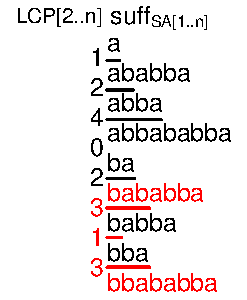
\includegraphics[width=0.2\textwidth,page=1]{sa+lcp+min.pdf}
    \end{center}
    \caption{\label{fig:sa+lcp+min}For $s=abbababba$, $\LCE(2,3)$ is the longest common prefix of $bababba$ and $bbababba$. There are two other suffixes between these in the lexicographical ordering, and the longest common prefixes between each pair of neighbors are 3, 1 and 3. Therefore $\LCE(2,3)= \min ~ \{3, 1, 3\} = 1$.}
\end{figure}

Different algorithms exists for solving the RMQ problem, and we can solve it in optimal $O(1)$ time and $O(n)$ space. But like for the LCE problem, the asymptotically best RMQ solution may not be the best RMQ solution in practice. We examine the following RMQ solutions, where \RMQpq{p}{q} has $O(p)$ space and preprocessing time, and $O(q)$ query time:
\begin{samepage}
\begin{description}
\item[\RMQn] walks through the array directly in $O(n)$ time and does not use any preprocessing (except for transforming LCE into RMQ).
\item[\RMQq] preprocesses the array in $O(n)$ space in order to do queries in $O(1)$ time. This is a twolevel data structure as shown in \pref{fig:sa+lcp+min-twolevel}. The array is split into blocks of size $O(\log n)$. The top level is an array of length $O(n/\log n)$, where each element contains the minimum value one block. The top level uses a \RMQpq{n\log n}{1}-solution, and the lower level precomputes all answers for each block, which is done in $O(n)$ space, since there are only a limited number of different block types of size $O(\log n)$.
\item[\RMQlog] is the same as \RMQq\ except that the lower level is replaced with a direct search through a $O(\log n)$ length block.
\end{description}
\end{samepage}

\begin{figure}[tp]
    \begin{center}
        \includegraphics[width=0.8\textwidth,page=2]{sa+lcp+min.pdf}
    \end{center}
    \caption{\label{fig:sa+lcp+min-twolevel}Twolevel Range Minimum Query. The range minimum is calculated as the minimum of one query in the top level and two queries in the lower level.}
\end{figure}

%%%%%%%%%%%%%%%%%%%%%%%%%%%%%%%%%%%%%%%%%%%%%%%%%%%%%%%%%%%%%%%%%%%%%%%%%%%%%%%
\subsubsection{Combining \proc{DirectComp} and \proc{LcpRmq}\label{sec:dc-lcprmq}}

Ilie~et~al.~\cite{ilie-navarro-tinta} suggests combining \proc{DirectComp} and \RMQn, by using \RMQn\ whenever the two suffixes we want to compare are close to each other in SA, and otherwise use \proc{DirectComp}. However that still gives $O(n)$ worst case query time. For example in the string $s=aaaaa...$, the query $\LCE(1,n/2)$ would require $\Omega(n)$ time for both \proc{DirectComp} and \RMQn.

We can instead combine \proc{DirectComp} and \RMQq, which we call \proc{DirectComp+LcpRmq}. \proc{DirectComp+LcpRmq} first uses \proc{DirectComp} until a specific cutoff and then switches over to \RMQq\ instead. This could have both the good average case query time of \proc{DirectComp} and the good worst case query time of \proc{LcpRmq}. However it still keeps the large space requirements of \proc{LcpRmq}, and it is not simple to implement like \proc{DirectComp}.

%%%%%%%%%%%%%%%%%%%%%%%%%%%%%%%%%%%%%%%%%%%%%%%%%%%%%%%%%%%%%%%%%%%%%%%%%%%%%%%
\subsection{The \proc{DirectCompLookup} Algorithm}

The input to the $LCE$ problem is two numbers $1 \leq i < j \leq n$ \footnote{We can assume that $i< j$ without loss of generality, since $\LCE(i,j)=\LCE(j,i)$}, so there are $n\cdot(n-1)/2 = O(n^2)$ different input possibilities in total. Because of this limited space of possible query inputs, we can tabulate a number of LCE values, and use those to speed up queries.

%%%%%%%%%%%%%%%%%%%%%%%%%%%%%%%%%%%%%%%%%%%%%%%%%%%%%%%%%%%%%%%%%%%%%%%%%%%%%%%
\subsubsection{\proc{DirectLookup}}

We can store results for all $O(n^2)$ possible queries in $O(n^2)$ space, and a query will then be a single table lookup in $O(1)$ time. We call this algorithm \proc{DirectLookup}. A result space table for \proc{DirectLookup} is shown in \pref{fig:resultspace-empty}, and \pref{fig:resultspace-directcomp} shows how \proc{DirectComp} moves through that table.

We can preprocess the table in in $O(n^2)$ time, since each value can be calculated in constant time like follows, if $LCE(i+1,j+1)$ is always calculated before $LCE(i,j)$ for any $i$ and $j$:
\begin{align*}
LCE(i,j) &=
\begin{cases}
    0 & \textrm{if} ~ s[i] \neq s[j] \\
    1 & \textrm{if} ~ s[i] = s[j] \wedge (i = n \lor j = n) \\
    LCE(i+1, j+1) + 1 & \textrm{otherwise} \\
\end{cases}
\end{align*}

\begin{figure}[tp]
    \begin{center}
        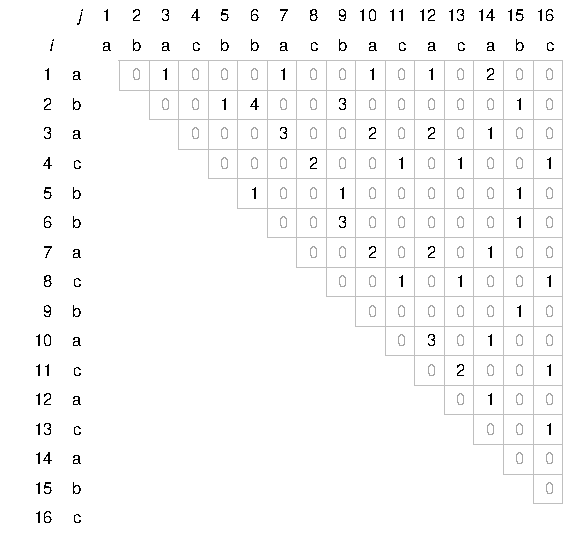
\includegraphics[width=0.5\textwidth,page=1]{resultspace.pdf}
    \end{center}
    \caption{\label{fig:resultspace-empty}The result space for $LCE_s(i,j)$ for $1 \leq i < j \leq n$ where $s = abacbbacbacacabc$.}
\end{figure}

\begin{figure}[tp]
    \begin{center}
        \includegraphics[width=0.5\textwidth,page=2]{resultspace.pdf}
    \end{center}
    \caption{\label{fig:resultspace-directcomp}$LCE(3,7)$ using \proc{DirectComp}.}
\end{figure}

%%%%%%%%%%%%%%%%%%%%%%%%%%%%%%%%%%%%%%%%%%%%%%%%%%%%%%%%%%%%%%%%%%%%%%%%%%%%%%%
\subsubsection{\proc{DirectComp} and \proc{DirectLookup} Combined}

\proc{DirectComp} and \proc{DirectLookup} preprocesses and stores no results and all results respectively. If we only store some results, we can use \proc{DirectComp} until we reach a stored result, and then retrieve this result using \proc{DirectLookup}. If we store every $t$'th row, as shown in \pref{fig:resultspace-t-row}, the space usage will be $O(n^2/t)$ and the worst case query time will be $O(t)$. We call this algorithm \proc{DirectCompLookup}.

\begin{figure}[tp]
    \begin{center}
        \includegraphics[width=0.5\textwidth,page=3]{resultspace.pdf}
    \end{center}
    \caption{\label{fig:resultspace-t-row}$LCE(3,7)$ with distance $t=4$ between each stored row.}
\end{figure}

%%%%%%%%%%%%%%%%%%%%%%%%%%%%%%%%%%%%%%%%%%%%%%%%%%%%%%%%%%%%%%%%%%%%%%%%%%%%%%%
\subsection{The \fprintk\ Algorithm}

\fi % report

\ifarticle
\section{The \fprintk\ Algorithm}
\fi % article

Our \fprintk\ algorithm generalizes \proc{DirectComp}. It compares characters starting at positions $i$ and $j$, but instead of comparing individual characters, it compares fingerprints of substrings. Given fingerprints of all substrings of length $t$, our algorithm can compare two $t$-length substrings in constant time.

%%%%%%%%%%%%%%%%%%%%%%%%%%%%%%%%%%%%%%%%%%%%%%%%%%%%%%%%%%%%%%%%%%%%%%%%%%%%%%%
\subsubsection{Definition of a Fingerprint}

Given a string $s$, the fingerprint $F_t[i]$ is a natural number identifying the substring $s[i\twodots i+t]$ among all $t$-length substrings of $s$. We assign fingerprints such that for any $i$, $j$ and $t$, $F_t[i] = F_t[j]$ if and only if $s[i\twodots i+t] = s[j\twodots j+t]$. In other words, if two substrings of $s$ have the same length, they have the same fingerprints if and only if the substrings themselves are the same.

At the end of a string when $i+t>n$, we define $F_t[i]$ by adding extra characters to the end of the string as needed.

%%%%%%%%%%%%%%%%%%%%%%%%%%%%%%%%%%%%%%%%%%%%%%%%%%%%%%%%%%%%%%%%%%%%%%%%%%%%%%%
\subsubsection{Data Structure\label{sec:fingerprint-ds}}

The \fprintk\ data structure for a string $s$ of length $n$, where $k$ is a parameter $1 \leq k \leq \logceil$, consists of $k$ natural numbers $t_0$, ..., $t_{k-1}$ and $k$ tables $H_0$, ..., $H_{k-1}$, each of length $n$. For each $\ell$ where $0\leq \ell\leq k-1$, $t_\ell = \Theta(n^{\ell/k})$ and table $H_\ell$ contains fingerprints of all $t_\ell$-length substrings of $s$, such that $H_\ell[i] = F_{t_\ell}[i]$. We always have $t_0 = n^{0/k} = 1$, such that $H_0$ is the original string $s$. The last character of the string must be a special character \$, which does not occur anywhere else in the string. An example is shown in \pref{fig:fingerprint-ds}.

\begin{figure}[tp]
    \begin{center}
        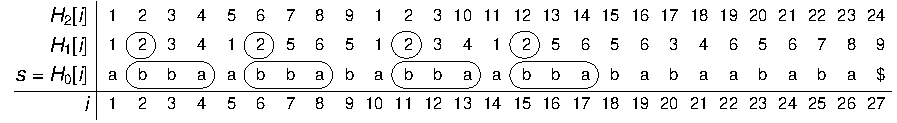
\includegraphics[width=0.98\textwidth,page=1]{fingerprint.pdf}
    \end{center}
    \caption{\label{fig:fingerprint-ds}\fprintk\ data structure for $s=\textit{abbaabbababbaabbababaababa\$}$, $n=27$, $k=3$, $t_1=n^{1/3}=3$ and $t_2=n^{2/3}=9$. All substrings $\textit{bba}$ are highlighted with their $3$-length fingerprint $2$.}
\end{figure}

\begin{lemma}
The \fprintk\ data structure takes $O(k\cdot n)$ space.
\end{lemma}
\begin{proof}
Each of the $k$ tables stores $n$ fingerprints of constant size.
\end{proof}

%%%%%%%%%%%%%%%%%%%%%%%%%%%%%%%%%%%%%%%%%%%%%%%%%%%%%%%%%%%%%%%%%%%%%%%%%%%%%%%
\subsubsection{Query\label{sec:fingerprint-query}}

To perform an LCE query using the \fprintk\ data structure, start with $v=0$ and $\ell=0$, then do the following steps:
\begin{samepage}
\begin{enumerate}
\item As long as $H_\ell[i+v] = H_\ell[j+v]$, increment $v$ by $t_\ell$, increment $\ell$ by one, and repeat this step unless and $\ell = k-1$.
\item As long as $H_\ell[i+v] = H_\ell[j+v]$, increment $v$ by $t_\ell$ and repeat this step.
\item When $H_\ell[i+v] \neq H_\ell[j+v]$, decrement $\ell$ by one and repeat step 2.
\item Stop when $\ell = 0$ and $H_\ell[i+v] \neq H_\ell[j+v]$.
\end{enumerate}

The LCE value is now $v = \LCE(i,j)$. An example is shown in \pref{fig:fingerprint-query}.
\end{samepage}

\begin{figure}[tp]
    \begin{center}
        \includegraphics[width=0.98\textwidth,page=2]{fingerprint.pdf}
    \end{center}
    \caption{\label{fig:fingerprint-query}\fprintk\ query for $\LCE(3,12)$ on the data structure of \pref{fig:fingerprint-ds}. The top half shows how $H_\ell[i+v]$ moves through the data structure, and the bottom half shows $H_\ell[j+v]$.}
\end{figure}

\begin{lemma}
The \fprintk\ query algorithm given above finds the correct LCE value.
\end{lemma}
\begin{proof}
At each step of the algorithm $v \leq \LCE(i,j)$, since the algorithm only increments $v$ by $t_\ell$ when it has found two matching fingerprints, and fingerprints of two substrings of the same length are only equal if the substrings themselves are equal. When the algorithm stops, it has found two fingerprints, which are not equal, and the length of these substrings is $t_\ell = 1$, therefore $v = \LCE(i,j)$.

The algorithm never reads $H_\ell[x]$, where $x>n$, because the string contains a unique character \$ at the end. This character will be at different positions in the substrings whose fingerprints are the last $t_\ell$ elements of $H_\ell$. These $t_\ell$ fingerprints will therefore be unique, and the algorithm will not continue at level $\ell$ after reading one of them.
\end{proof}

\begin{lemma}
The worst case query time for \fprintk\ is $O(k\cdot n^{1/k})$, and the average case query time is $O(1)$.
\end{lemma}
\begin{proof}
Step 1 takes $O(k)$ time. In step 2 and 3, the number of remaining characters left to check at level $\ell$ is $O(n^{(\ell+1)/k})$, since the previous level found two differing substrings of that length (at the top level $\ell=k-1$ we have $O(n^{(\ell+1)/k}) = O(n)$). Since we can check $t_\ell = \Theta(n^{\ell/k})$ characters in constant time at level $\ell$, the algorithm uses $O(n^{(\ell+1)/k})/\Theta(n^{\ell/k}) = O(n^{1/k})$ time at that level. Over all $k$ levels, $O(k\cdot n^{1/k})$ query time is used.

At each step except step 3, the algorithm increments $v$. Step 3 is executed the same number of times as step 1, in which $v$ is incremented. The query time is therefore linear to the number of times $v$ is incremented, and it is thereby $O(v)$. The query time is thus $O(1)$ in average case, where $v=O(1)$.
\end{proof}

%%%%%%%%%%%%%%%%%%%%%%%%%%%%%%%%%%%%%%%%%%%%%%%%%%%%%%%%%%%%%%%%%%%%%%%%%%%%%%%
\subsubsection{Average Case Optimization\label{sec:improved-avg}}

We could have left out step 1 of the query algorithm in \pref{sec:fingerprint-query} and started with $\ell=k-1$, which would change the query pattern as shown in \pref{fig:fingerprint-updown}. This would keep the asymptotic worst case query time of $O(k\cdot n^{1/k})$, but it would increase our average case query time to $O(k)$. Our experiments have shown that whenever $k$ is small, keeping step 1 improves average case query time, while it does not have a measurable effect on worst case query times. When $k = \logceil$, keeping step 1 can double the worst case query time, while it can make the average case query time 40 times faster for an input string of ten million characters. We want to optimize our LCE query time for the average case where the LCE value is small, so our results in \pref{sec:results} does not include the variant of \fprintk\ with $O(k)$ average case query time.

In step 1 of our query algorithm we perform one comparison at each level. We could instead do up to $O(n^{1/k})$ comparisons at each level without affecting asymptotic times. Our experiments have shown that always doing one comparison at each level is the best in practice.

\begin{figure}[tp]
    \begin{center}
        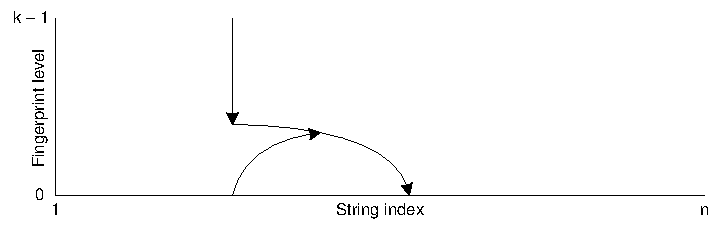
\includegraphics[width=1\textwidth,page=1]{fingerprint-updown.pdf}
    \end{center}
    \caption{\label{fig:fingerprint-updown}Two ways of querying the fingerprint levels, one starting from level $\ell=k-1$ and one starting at level $\ell=0$.}
\end{figure}

%%%%%%%%%%%%%%%%%%%%%%%%%%%%%%%%%%%%%%%%%%%%%%%%%%%%%%%%%%%%%%%%%%%%%%%%%%%%%%%
\subsubsection{Preprocessing}

The tables of fingerprints use $O(k\cdot n)$ space. In the case with $k=\logceil$ levels, the data structure is the one generated by Karp-Miller-Rosenberg~\cite{karp-miller-rosenberg}. This data structure can be constructed in $O(n\log n)$ time. With $k<\logceil$ levels, KMR can be adapted, but it still uses $O(n\log n)$ preprocessing time.

We can preprocess the data structure in $O(\sortt + k\cdot n)$ time using the SA and LCP arrays. First create the SA and LCP arrays. Then preprocess each of the $k$ levels using the following steps:
\begin{samepage}
\begin{enumerate}
\item Loop through the $n$ substrings of length $t_\ell$ in lexicographically sorted order by looping through the elements of SA.
\item Assign an arbitrary fingerprint to the first substring.
\item If the current substring $s[\SA[i]\twodots\SA[i]+t_\ell]$ is equal to the substring examined in the previous iteration of the loop, give the current substring the same fingerprint as the previous substring, otherwise give the current substring a new unused fingerprint. The two substrings are equal when $\LCE[i] \geq t_\ell$.
\end{enumerate}

An example is shown in \pref{fig:fingerprint-preproc}.
\end{samepage}

\begin{figure}[tp]
    \begin{center}
        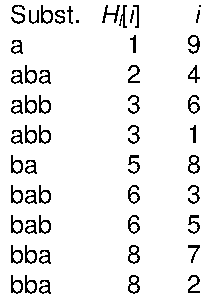
\includegraphics[width=0.2\textwidth,page=1]{fingerprint-preproc.pdf}
    \end{center}
    \caption{\label{fig:fingerprint-preproc}The first column lists all substrings of $s=abbababba$ with length $t_\ell = 3$. The second column lists fingerprints assigned to each substring. The third column lists the position of each substring in $s$.}
\end{figure}

\begin{lemma}
The preprocessing algorithm described above generates the data structure described in \pref{sec:fingerprint-ds}.
\end{lemma}

\begin{proof}
We always assign two different fingerprints whenever two substrings are different, because whenever we see two differing substrings, we change the fingerprint to a value not previously assigned to any substring.

We always assign the same fingerprint whenever two substrings are equal, because all substrings, which are equal, are grouped next to each other, when we loop through them in lexicographical order.
\end{proof}

\begin{lemma}
The preprocessing algorithm described above takes $O(\sortt + k\cdot n)$ time.
\end{lemma}

\begin{proof}
We first construct the SA and LCP arrays, which takes $O(\sortt)$ time~\cite{sort-complexity}. We then preprocess each of the $k$ levels in $O(n)$ time, since we loop through $n$ substrings, and comparing neighboring substrings takes constant time when we use the LCE array. The total preprocessing time becomes $O(\sortt + k\cdot n)$.
\end{proof}

\ifreport

%%%%%%%%%%%%%%%%%%%%%%%%%%%%%%%%%%%%%%%%%%%%%%%%%%%%%%%%%%%%%%%%%%%%%%%%%%%%%%%
\subsubsection{Cache Optimization\label{sec:fingerprint-cache}}

\paragraph{Horizontal, intra-level optimization}

The amount if I/O's used by \fprintk\ is $O(k\cdot n^{1/k})$. However if we structure our tables of fingerprints differently, we can improve the number of I/O's to $O(k(n^{1/k}/B+1))$ in the cache-oblivious model. Instead of storing the fingerprint of $s[i\twodots i+t_\ell]$ at $H_\ell[i]$, we can store it at $H_\ell[((i-1)\mod t_\ell)\cdot\lceil n/t_\ell\rceil+\lfloor (i-1)/t_\ell\rfloor+1]$. This will group all used fingerprints at level $\ell$ next to each other in memory, such that the amount of I/O's at each level is reduced from $O(n^{1/k})$ to $O(n^{1/k}/B)$.

The size of each fingerprint table will grow from $|H_\ell| = n$ to $|H_\ell| = n+t_\ell$, because the rounding operations may introduce one-element gaps in the table after every $n/t_\ell$ elements. We achieve the greatest I/O improvement when $k$ is small. When $k=\logceil$, this cache optimization gives no difference in the amount of I/O's.

\paragraph{Vertical, inter-level optimization}

For larger values of $k$, we can attempt to optimize memory access accross different levels. When we move down through the levels for $k=\logceil$, we can continue in two directions after reading $H_\ell[i]$: $H_{\ell-1}[i]$ or $H_{\ell-1}[i+t_\ell]$. Neither of these positions are next to $H_\ell[i]$ in memory. We can optimize for the case where we reach $H_{\ell-1}[i]$ by flipping the direction in which we store the fingerprints, such that all fingerprints $H_\ell[i]$ for all $\ell$ and a specific $i$ are stored next to each other. This will not improve the asymptotic I/O bound, but could improve practical query times.

%%%%%%%%%%%%%%%%%%%%%%%%%%%%%%%%%%%%%%%%%%%%%%%%%%%%%%%%%%%%%%%%%%%%%%%%%%%%%%%
\subsection{Space Usage}

\pref{tab:algorithms-space} shows the space requirement of each of our analyzed algorithms. The size of the input string of $n/4$ words is not included, and we ignore constant terms.

\begin{table}[tp]
\centering
\begin{minipage}{0.7\textwidth}
\centering
\begin{tabular}{l|l}
\hline\hline
Algorithm & Space \\ [0.5ex] \hline
\proc{DirectComp} & $0$ words \\ \hline
\proc{DirectLookup} & $2n^2$ words \footnote{The factor two comes from using shift instead of multiplication, which may double the size depending on $n$.} \\ \hline
\proc{DirectCompLookup} & $2n^2/t+n$ words \\ \hline
\proc{LcpRmq} & ca. $5.6n$ words \footnote{Space use for \proc{LcpRmq} is $2n + 2nb + (bs \cdot (bs+1) / 2 + 1)\cdot C_{bs} + (nb+1)\cdot \lfloor\log nb\rfloor \approx 5.6n$, where $bs = \lceil\log n / 4\rceil$, $nb = (n-1)/bs+1$ and $C_i$ is the $i$'t Catalan Number.} \\ \hline
\fprint[2] & $n$ words \\ \hline
\fprint[3] & $2n$ words \\ \hline
\fprint[\logceil] & $n\cdot\logceil$ words \\ \hline
\end{tabular}
\end{minipage}
\caption{Space requirements for the LCE algorithms, where $n$ is the number of characters, a character is one byte and a word is four bytes.}\label{tab:algorithms-space}
\end{table}

\fi % report

%%%%%%%%%%%%%%%%%%%%%%%%%%%%%%%%%%%%%%%%%%%%%%%%%%%%%%%%%%%%%%%%%%%%%%%%%%%%%%%
%%%%%%%%%%%%%%%%%%%%%%%%%%%%%%%%%%%%%%%%%%%%%%%%%%%%%%%%%%%%%%%%%%%%%%%%%%%%%%%
\section{Experimental Results\label{sec:results}}

In this section we show results of actual performance measurements. The measurements were done on a Windows 23-bit machine with an Intel P8600 CPU (3 MB L2, 2.4 GHz) and 4 GB RAM. The code was compiled using GCC 4.5.0 with \texttt{-O3}.

%%%%%%%%%%%%%%%%%%%%%%%%%%%%%%%%%%%%%%%%%%%%%%%%%%%%%%%%%%%%%%%%%%%%%%%%%%%%%%%
\subsection{Tested Algorithms}

\ifarticle

We implemented different variants of the \fprintk\ algorithm in C++ and compared them with optimized versions of the \proc{DirectComp} and \proc{LcpRmq} algorithms. The algorithms we compared are the following:
\begin{description}
\item[\proc{DirectComp}] is the simple \proc{DirectComp} algorithm with no preprocessing and worst case $O(n)$ query time.
\item[\fprintk\textless$t_{k-1}$, ..., $t_1$\textgreater ac] is our new \fprintk\ algorithm using $k$ levels, where $k$ is $2$, $3$ and $\logceil$. The numbers \textless$t_{k-1}$, ..., $t_1$\textgreater describe the exact size of fingerprinted substrings at each level.
\item[\proc{RMQ}\textless$n$, $1$\textgreater] is the \proc{LcpRmq} algorithm using constant time RMQ.
\end{description}

\fi % article

\ifreport

We implemented different variants of \proc{DirectComp}, \proc{LcpRmq}, \proc{DirectCompLookup} and \fprintk\ in C++ and compared them to each other. We have not implemented \proc{SuffixNca}, since others have shown that \proc{LcpRmq} is better than \proc{SuffixNca} in practice~\cite{ilie-navarro-tinta}. The algorithms we compared are the following:
\begin{description}
\item[\proc{DirectComp}] is the simple \proc{DirectComp} algorithm with no preprocessing and worst case $O(n)$ query time.
\item[\fprintk\textless$t_{k-1}$, ..., $t_1$\textgreater ac] is our new \fprintk\ algorithm using $k$ levels, where $k$ is $2$, $3$ and $\logceil$. The numbers \textless$t_{k-1}$, ..., $t_1$\textgreater\ describe the exact size of fingerprinted substrings at each level.
\item[\fprintk\textless$t_{k-1}$, ..., $t_1$\textgreater wc] is a variant of our new \fprintk\ algorithm, which starts at level $\ell=k-1$ instead of $\ell=0$, as discussed in \pref{sec:improved-avg}.
\item[\fprintk\textless$t_{k-1}$, ..., $t_1$\textgreater ac\textless$u_0$, ..., $u_{k-2}$\textgreater] is a variant of our new \fprintk\ algorithm, which stays at level $\ell$ until $v\geq u_\ell$, as discussed in \pref{sec:improved-avg}, instead of doing one comparison at each level in step 1 of the query in \pref{sec:fingerprint-query}.
\item[\proc{RMQ}\textless$n$, $1$\textgreater] is the \proc{LcpRmq} algorithm using constant time RMQ.
\item[\proc{RMQ}\textless$p$, $q$\textgreater$_{\textrm{virtual}}$] is the \proc{LcpRmq} algorithm using different RMQ algorithms. They all contain an additional virtual method call to make implementation simpler, but their results cannot be directly compared to other algorithms, which do not have this extra virtual method call.
\item[\proc{DirectComp}\textless$c$\textgreater\proc{RMQ}\textless$n$, $1$\textgreater] is the \proc{DirectComp+LcpRmq} algorithm, where the cutoff from \proc{DirectComp} to \proc{LcpRmq} is after $c$ iterations.
\item[\fprintk\textless$t_{k-1}$, ..., $t_1$\textgreater ac$_{\textrm{cache-horizontal-}\textit{op}}$] is a cache optimized variant of our \fprintk\ algorithm, where \textit{op} describes which of the shift or multiplication arithmetic operations it uses.
\end{description}

\fi % report

%%%%%%%%%%%%%%%%%%%%%%%%%%%%%%%%%%%%%%%%%%%%%%%%%%%%%%%%%%%%%%%%%%%%%%%%%%%%%%%
\subsection{Test Inputs and Setup}

We have tested the algorithms on different kinds of strings:
\begin{description}
\item[Average case strings] These strings have many small LCE values, such that the average LCE value over all $n^2$ query pairs is less than one. We use results on these strings as an indication average case query times over all input pairs $(i,j)$ in cases where most or all LCE values are small on expected input strings. We construct these strings by choosing each character uniformly at random from an alphabet of size 10
\item[Worst case strings] These strings have many large LCE values, such that the average LCE value over all $n^2$ query pairs is $n/2$. We use results on these strings as an indication of worst case query times, since the query times for all tested algorithms are asymptotically at their worst when the LCE value is large. We construct these strings with an alphabet size of one.
\item[Medium LCE value strings] These strings have an average LCE value over all $n^2$ query pairs of $n/2r$, where $r=0.73n^{0.42}$. We use results on these strings as an indication of query times somewhere between the average case and worst case. We construct these strings by repeating a substring of $r$ characters, where each character is unique.
\end{description}

For each kind of strings, we tested the algorithms using the following pattern:
\begin{enumerate}
\item Generate a string of length $n$ and generate a million random pairs $(i, j)$, where each of $i$ and $j$ is chosen between $1$ and $n$ uniformly at random.
\item For each tested algorithm, preprocess the given string, and run a query for each of the million pairs. Measure the time it takes to run all the queries combined.
\item Double the value of $n$ and repeat from step 1.
\end{enumerate}

\ifreport

%%%%%%%%%%%%%%%%%%%%%%%%%%%%%%%%%%%%%%%%%%%%%%%%%%%%%%%%%%%%%%%%%%%%%%%%%%%%%%%
\subsection{\proc{LcpRmq} Results\label{sec:test-rmq}}

We want to compare our new algorithms against the algorithm which is the best in practice of the asymptotically best $O(1)$ algorithms. The \proc{LcpRmq} algorithm is better than \proc{SuffixNca}~\cite{ilie-navarro-tinta}, so we only look at \proc{LcpRmq}. We have looked at a number of RMQ algorithms to find out which works best for the LCE problem. The results are shown in \pref{fig:plot-rmq}. \RMQq\ is the best in practice, and we therefore use that when we test against other LCE algorithms. This result is different from that of Ilie~et~al.~\cite{ilie-navarro-tinta}, where \RMQpq{n}{4\log n} is the best. This could be due to hardware or compiler differences.

The performance of the implementations shown in \pref{fig:plot-rmq} cannot be compared with those shown on other figures, because they all contain an additional, slow virtual method call, which gives them an unfair disadvantage. We have optimized the best variant of \proc{LcpRmq} to avoid the virtual method call, when we compare it against other algorithms. We compare this optimized version to \proc{DirectComp} in \pref{fig:plot-rmq-directcomp}, which shows that \proc{DirectComp} is significantly better in average case, though both have constant asymptotic average case query times.

The RMQ algorithms show a significant jump in query times around $n=1.000.000$ on the plot with average case strings, but not on the plot with worst case strings. We have run the tests in Cachegrind, and found that the number of instructions executed and the number of data reads and writes are exactly the same for both average case strings and worst case strings. The cache miss rate for \RMQq\ on average case strings is 14\% and 9\% for the L1 and L2 caches, and on worst case strings the miss rate is 17\% and 13\%, which is the opposite of what could explain the jump we see in the plot.

% size = 3,5*2^30 = 3758096384
% assoc = (3,5*2^30)/(4*2^10) = 917504
% line = 4*2^10 = 4096
% --LL=3758096384,917504,4096

% size = 1*2^30 = 1073741824
% assoc = (1*2^30)/(4*2^10) = 262144
% line = 4*2^10 = 4096
% --LL=1073741824,262144,4096

\begin{figure}[tp]
    \begin{center}
        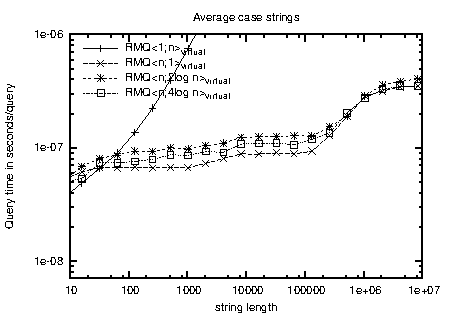
\includegraphics[width=0.49\textwidth,type=pdf,ext=.pdf,read=.pdf]{../src/results/length-rmq-rand10.plt}
        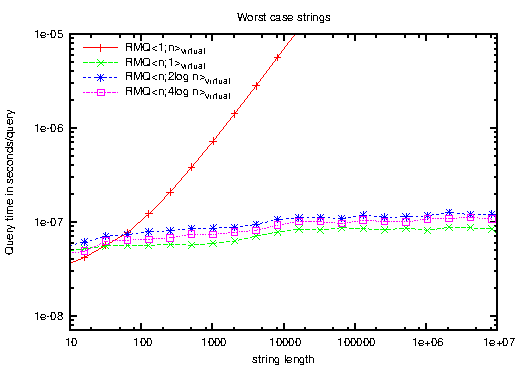
\includegraphics[width=0.49\textwidth,type=pdf,ext=.pdf,read=.pdf]{../src/results/length-rmq-alla.plt}
    \end{center}
    \caption{\label{fig:plot-rmq}Query times of \proc{LcpRmq} using different variants of RMQ.}
\end{figure}

%%%%%%%%%%%%%%%%%%%%%%%%%%%%%%%%%%%%%%%%%%%%%%%%%%%%%%%%%%%%%%%%%%%%%%%%%%%%%%%
\subsubsection{\proc{DirectComp+LcpRmq} Results}

\pref{fig:plot-rmq-directcomp} also shows \proc{DirectComp+LcpRmq}, where we first try \proc{DirectComp}, and if we have not found the LCE value after one iteration, we use \proc{LcpRmq} instead. We see that \proc{DirectComp+LcpRmq} is worse than \proc{DirectComp} on average case strings. We could increase the cutoff from one iteration to something bigger, which might improve average case performance. That would however increase worst case time. None of the two plots we measure represents a good worst case for \proc{DirectComp+LcpRmq} compared to the other algorithms we test. The worst case for \proc{DirectComp+LcpRmq} relative to other the other algorithms would be when the average LCE value is slightly larger than the cutoff, such that \proc{DirectComp+LcpRmq} reaches \proc{LcpRmq} in most queries, while other algorithms still work on LCE values as small as possible. As described in \pref{sec:dc-lcprmq}, \proc{DirectComp+LcpRmq} also uses a lot of space.

\begin{figure}[tp]
    \begin{center}
        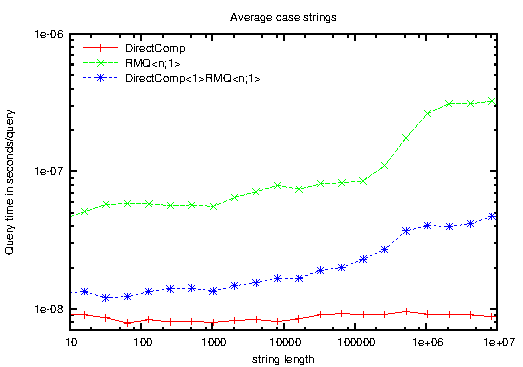
\includegraphics[width=0.49\textwidth,type=pdf,ext=.pdf,read=.pdf]{../src/results/length-rmq-directcomp-rand10.plt}
        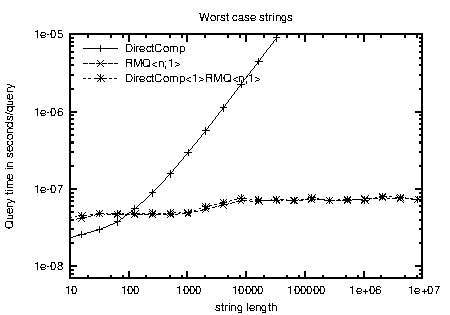
\includegraphics[width=0.49\textwidth,type=pdf,ext=.pdf,read=.pdf]{../src/results/length-rmq-directcomp-alla.plt}
    \end{center}
    \caption{\label{fig:plot-rmq-directcomp}Query times of constant time \proc{LcpRmq}, \proc{DirectComp} and \proc{DirectComp+LcpRmq}.}
\end{figure}

%%%%%%%%%%%%%%%%%%%%%%%%%%%%%%%%%%%%%%%%%%%%%%%%%%%%%%%%%%%%%%%%%%%%%%%%%%%%%%%
\subsection{\proc{DirectCompLookup} Results}


\pref{fig:plot-complookup} shows \proc{DirectCompLookup} with different time/space-tradeoffs together with \proc{LcpRmq}. In average case, \proc{DirectCompLookup} is slower than \proc{DirectComp}, most likely because it needs to do an extra check to find out if it has reached a position for which a result is stored. For short strings, \proc{DirectLookup} is faster than \proc{DirectCompLookup}, since it does not need to check if the value it needs is stored. However, it quickly grows to be as slow as \proc{LcpRmq}, while \proc{DirectCompLookup} does not experience this slowdown. We explain this with that \proc{DirectLookup} reads from its $O(n^2)$ table of results in every query, whereas \proc{DirectCompLookup} only reads from the $O(n)$ string in average case, and thus has a significantly smaller working set.

In the worst case, the \proc{DirectCompLookup} variants which use more space are faster in practice, just like in theory. If we are willing to use $O(n\log n)$ space, \proc{DirectCompLookup}\textless$n/\log n$\textgreater\ will only halve the worst case query time compared to \proc{DirectComp}. This makes \proc{DirectCompLookup} better than \proc{DirectComp}, but still not a very good candidate when worst case query time is important.

\proc{DirectCompLookup} uses $O(n^2)$ preprocessing time no matter what parameter $t$ we choose, which is significantly slower than any of the other algorithms we have tested, and it is also the reason why we have only tested this algorithm up until $n=100.000$. The only way we have found to improve this preprocessing time is to use one of the other algorithms we have covered to preprocess the data structure of \proc{DirectCompLookup}.

\begin{figure}[tp]
    \begin{center}
        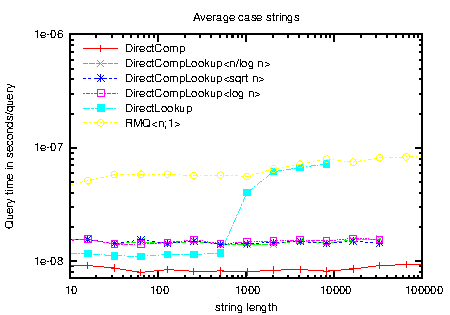
\includegraphics[width=0.49\textwidth,type=pdf,ext=.pdf,read=.pdf]{../src/results/length-complookup-rand10.plt}
        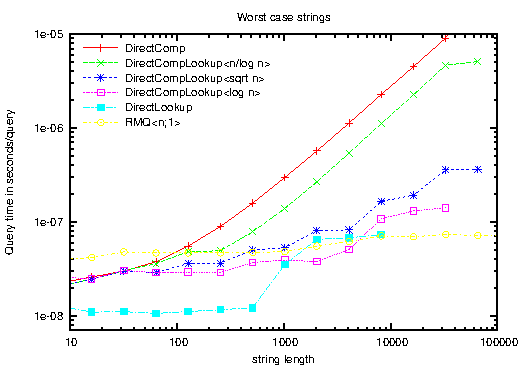
\includegraphics[width=0.49\textwidth,type=pdf,ext=.pdf,read=.pdf]{../src/results/length-complookup-alla.plt}
    \end{center}
    \caption{\label{fig:plot-complookup}Query times of our new DirectCompLookup algorithm versus the existing \proc{DirectComp} and \proc{LcpRmq} algorithms.}
\end{figure}

%%%%%%%%%%%%%%%%%%%%%%%%%%%%%%%%%%%%%%%%%%%%%%%%%%%%%%%%%%%%%%%%%%%%%%%%%%%%%%%
\subsection{\fprintk\ Results}

\fi % report

\ifarticle
\subsection{Results}
\fi % article

\begin{figure}[tp]
    \begin{center}
        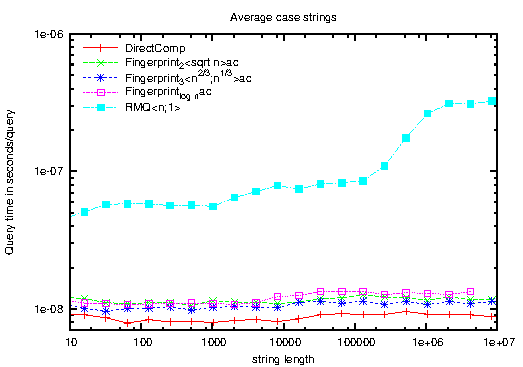
\includegraphics[width=0.7\textwidth,type=pdf,ext=.pdf,read=.pdf]{../src/results/length-article-rand10.plt}
        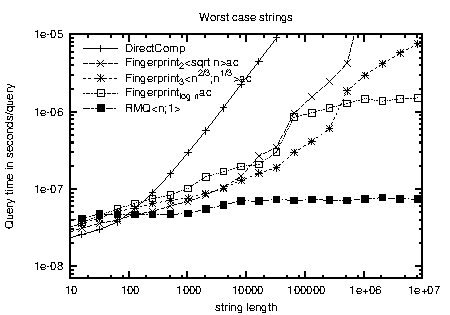
\includegraphics[width=0.7\textwidth,type=pdf,ext=.pdf,read=.pdf]{../src/results/length-article-alla.plt}
        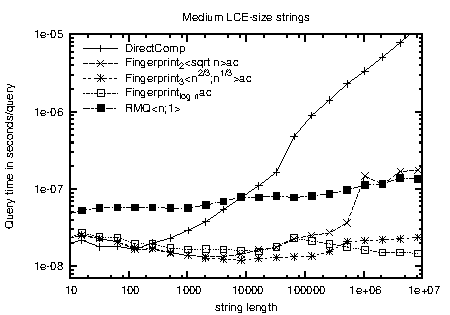
\includegraphics[width=0.7\textwidth,type=pdf,ext=.pdf,read=.pdf]{../src/results/length-article-repeat-pow.plt}
    \end{center}
    \caption{\label{fig:test-fingerprint}Comparison of our new \fprintk\ algorithm for $k=2$, $k=3$ and $k=\logceil$ versus the existing \proc{DirectComp} and \proc{LcpRmq} algorithms.}
\end{figure}

\begin{table}[tp]
\centering
\begin{tabular}{l|r|r|r|r|r|r|r}
\hline\hline
% File & \proc{DirectComp} & \fprint[2]\textless$\sqrt n$\textgreater ac & \fprint[3]\textless$n^{2/3}$, $n^{1/3}$\textgreater ac & \fprint[\log n]ac & RMQ<n;1> \\ [0.5ex] \hline
File & $n$ & $\sigma$ & DC & FP$_2$ & FP$_3$ & FP$_{\log n}$ & RMQ \\ [0.5ex] \hline
book1 & $0.7\cdot 2^{20}$ & 82 & 8.1 & 11.4 & 10.6 & 12.0 & 218.0 \\ \hline
kennedy.xls & $1.0\cdot 2^{20}$ & 256 & 11.9 & 16.0 & 16.1 & 18.6 & 114.4 \\ \hline
E.coli & $4.4\cdot 2^{20}$& 4 & 12.7 & 16.5 & 16.6 & 19.2 & 320.0 \\ \hline
bible.txt & $3.9\cdot 2^{20}$ & 63 & 8.5 & 11.3 & 10.5 & 12.6 & 284.0 \\ \hline
world192.txt & $2.3\cdot 2^{20}$ & 93 & 7.9 & 10.5 & 9.8 & 12.7 & 291.7 \\ \hline
\end{tabular}
\caption{Query times in nano seconds for \proc{DirectComp} (DC), \fprintk\ (FP$_k$) and \proc{LcpRmq} (RMQ) on the five largest files from the Canterbury corpus.}\label{tab:text-fprint-files}
\end{table}

\pref{fig:test-fingerprint} shows our experimental results on average case strings with a small average LCE value, worst case strings with a large average LCE value, and strings with a medium average LCE value.

On average case strings, our new \fprintk\ algorithm is approximately 20\% slower than \proc{DirectComp}, and it is between than 5 and 25 times faster than \proc{LcpRmq}. We see the same results on some real world strings in \pref{tab:text-fprint-files}.

On worst case strings, the \fprintk\ algorithms are significantly better than \proc{DirectComp} and somewhat worse than \proc{LcpRmq}. Up until $n=30.000$ the three measured \fprintk\ algorithms have nearly the same query times. Of the \fprintk\ algorithms, the $k=2$ variant has a slight advantage for small strings of length less than around $2.000$. For longer strings the $k=3$ variant performs the best up to strings of length $250.000$, at which point the $k=\logceil$ variant becomes the best. This indicates that for shorter strings, using fewer levels is better, and when the input size increases, the \fprintk\ variants with better asymptotic query times have better worst case times in practice.

On strings with medium average LCE values, we see that our \fprintk\ algorithms are faster than both \proc{DirectComp} and \proc{LcpRmq}

We conclude that our new \fprintk\ algorithm achieves a tradeoff between worst case times and average case times, which is better than the existing best \proc{DirectComp} and \proc{LcpRmq} algorithms, yet it is not strictly better than the existing algorithms on all inputs. \fprintk\ is therefore a good choice in cases where both average case and worst case performance is important.

%  \fprint[3]\ also shows such a jump, but for greater input sizes, as it uses less memory.

\ifarticle

\proc{LcpRmq} shows a significant jump in query times around $n=1.000.000$ on the plot with average case strings, but not on the plot with worst case strings. We have run the tests in Cachegrind, and found that the number of instructions executed and the number of data reads and writes are exactly the same for both average case strings and worst case strings. The cache miss rate for average case strings is 14\% and 9\% for the L1 and L2 caches, and for worst case strings the miss rate is 17\% and 13\%, which is the opposite of what could explain the jump we see in the plot.

\fi % article

% \fixme{Results: Investigate if we can explain the jump in Fingerprint-log}
% \paragraph{\fprint[\log n] cache limit.}
% \proc{LcpRmq} uses more space than all of \proc{DirectComp}, \fprint[2] and \fprint[3], so it is expected that it reaches the cache limit before these. However \fprint[\log n] uses more space than \proc{LcpRmq} at the input sizes we measure, since \proc{LcpRmq} uses the same amount of memory as \fprint[6], and $\lceil\log(10.000.000)\rceil = 24$. However, the \fprintk\ algorithms only access the lowest levels of their data structure whenever the LCE values are small, and there is therefore no visible jump due to cache limits for \fprint[\log n] on the plot with average case strings. On the plot with worst case strings however, we see a jump in \fprint[\log n] between $n=20.000$ and $n=50.000$, since it uses all its $\logceil$ levels when the LCE values are large.

\ifreport

%%%%%%%%%%%%%%%%%%%%%%%%%%%%%%%%%%%%%%%%%%%%%%%%%%%%%%%%%%%%%%%%%%%%%%%%%%%%%%%
\subsubsection{Optimal Value of $t_\ell$}

\pref{fig:plot-fingerprint-tval} shows \fprint[2] for different values of $t_1$. On average case strings the value of $t_1$ makes no difference, and on worst case strings a value of $t_1$ between $2\sqrt n$ and $4\sqrt n$ is the best. The improvement relative to $\sqrt n$ is however insignificant, so we have chosen to use $t_1=\sqrt n$.

Our results indicate that reading values from $H_0$ is faster than reading values from $H_1$. Differences between these two tables include that elements of $H_0 = s$ use one byte, whereas elements of $H_1$ use four bytes, and that elements we read from $H_0$ are located next to each other in memory, whereas elements we read from $H_1$ are spaced $t_1$ elements apart in memory.

\begin{figure}[tp]
    \begin{center}
        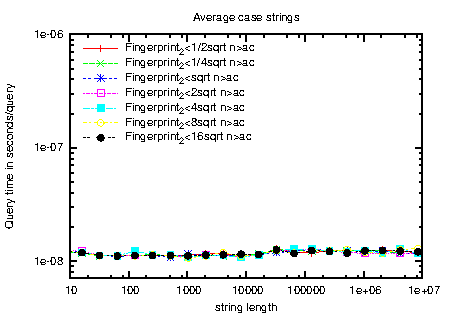
\includegraphics[width=0.49\textwidth,type=pdf,ext=.pdf,read=.pdf]{../src/results/length-fingerprint-2l-rand10.plt}
        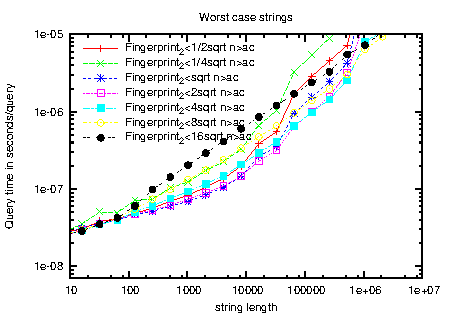
\includegraphics[width=0.49\textwidth,type=pdf,ext=.pdf,read=.pdf]{../src/results/length-fingerprint-2l-alla.plt}
    \end{center}
    \caption{\label{fig:plot-fingerprint-tval}Query times of \fprint[2] for different values of $t_1$ versus query times for \proc{DirectComp}.}
\end{figure}


%%%%%%%%%%%%%%%%%%%%%%%%%%%%%%%%%%%%%%%%%%%%%%%%%%%%%%%%%%%%%%%%%%%%%%%%%%%%%%%
\subsubsection{Average Case Optimization\label{sec:test-average}}

In \pref{sec:improved-avg} we discussed how our \fprintk\ algorithm is optimized for the average case to get $O(1)$ instead of $O(k)$ average case query time, while it keeps the same asymptotic worst case query time. But in practice the worst case query time is slightly affected.

\begin{figure}[tp]
    \begin{center}
        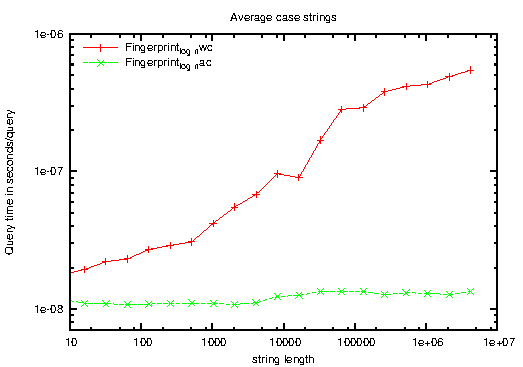
\includegraphics[width=0.49\textwidth,type=pdf,ext=.pdf,read=.pdf]{../src/results/length-fingerprint-avglog-rand10.plt}
        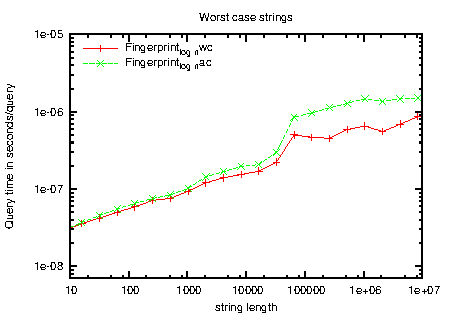
\includegraphics[width=0.49\textwidth,type=pdf,ext=.pdf,read=.pdf]{../src/results/length-fingerprint-avglog-alla.plt}
    \end{center}
    \caption{\label{fig:plot-fingerprint-avglog}Query times of \fprint[\logceil] with $O(1)$ versus $O(k)$ average case query time.}
\end{figure}

In \pref{fig:plot-fingerprint-avglog} we see that on worst case strings, the query time of \fprint[\logceil] degrade a small amount when using the average case optimization. Both variations of \fprint[\logceil] show query times, which are $O(\log n)$ as expected. On average case strings, the query time of \fprint[\logceil] improves significantly when using average case optimization, and both variants show their expected $O(1)$ and $O(\log n)$ average case query times.

\begin{figure}[tp]
    \begin{center}
        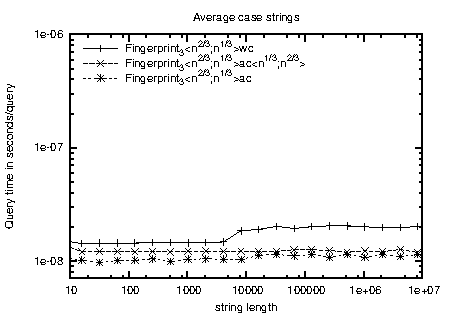
\includegraphics[width=0.49\textwidth,type=pdf,ext=.pdf,read=.pdf]{../src/results/length-fingerprint-avg3l-rand10.plt}
        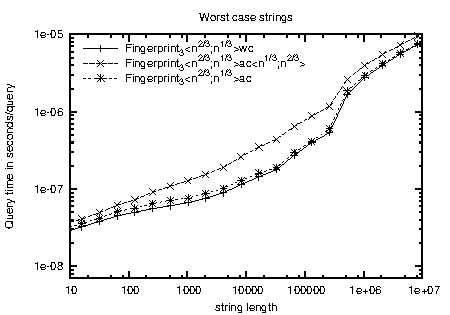
\includegraphics[width=0.49\textwidth,type=pdf,ext=.pdf,read=.pdf]{../src/results/length-fingerprint-avg3l-alla.plt}
    \end{center}
    \caption{\label{fig:plot-fingerprint-avg3l}Query times of \fprint[3] with $O(1)$ versus $O(k)$ average case query time.}
\end{figure}

In \pref{fig:plot-fingerprint-avg3l} we see that doing one comparison at each level on the way up is better than doing $n^{1/k}$ comparisons. This is most visible on worst case strings, where the algorithm doing one comparison at each level uses less time to reach level $\ell=k-1$, which it will reach anyway. On average case strings, the code specialized in handling only one comparison at each level is simpler. On the question of doing average case optimization or not, we see the same results for \fprint[3], as we saw for \fprint[\logceil], but at a smaller scale.

We conclude that using average case optimization yields a query time improvement on average case strings, which is significantly greater than the query time increase on worst case strings, and that \fprintk\ therefore should use the average case optimization.

%%%%%%%%%%%%%%%%%%%%%%%%%%%%%%%%%%%%%%%%%%%%%%%%%%%%%%%%%%%%%%%%%%%%%%%%%%%%%%%
\subsubsection{Cache Optimization}

\begin{figure}[tp]
    \begin{center}
        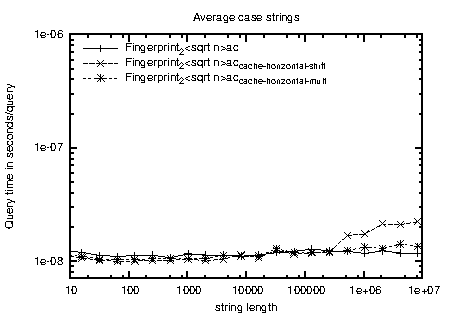
\includegraphics[width=0.49\textwidth,type=pdf,ext=.pdf,read=.pdf]{../src/results/length-fingerprint-cache-rand10.plt}
        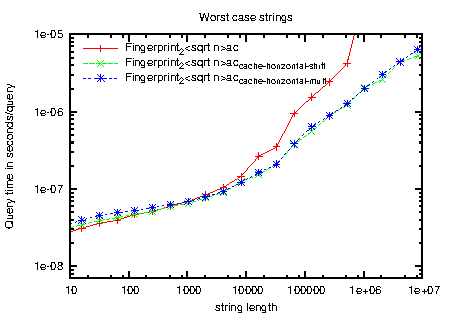
\includegraphics[width=0.49\textwidth,type=pdf,ext=.pdf,read=.pdf]{../src/results/length-fingerprint-cache-alla.plt}
        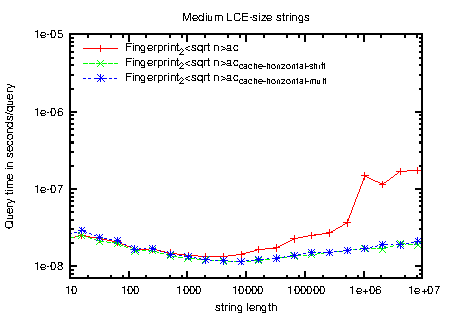
\includegraphics[width=0.49\textwidth,type=pdf,ext=.pdf,read=.pdf]{../src/results/length-fingerprint-cache-repeat-pow.plt}
        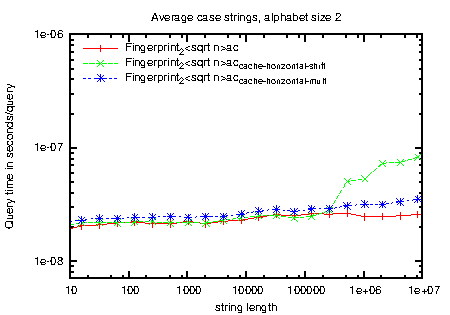
\includegraphics[width=0.49\textwidth,type=pdf,ext=.pdf,read=.pdf]{../src/results/length-fingerprint-cache-rand2.plt}
    \end{center}
    \caption{\label{fig:plot-fingerprint-cache-horiz}Query times of \fprint[2] with and without cache optimization.}
\end{figure}

\paragraph{Horizontal, intra-level optimization}

\pref{fig:plot-fingerprint-cache-horiz} shows results of the intra-level cache optimization described in \pref{sec:fingerprint-cache}. We have implemented two intra-level cache optimized variants. One as described in \pref{sec:fingerprint-cache}, and one where multiplication and division is replaced with shift operations. To use shift operations, $t_\ell$ and $\lceil n/t_\ell\rceil$ must both be powers of two. This may double the size of the used address space.

On average case strings the cache optimization does not change the query times, while on worst case strings and strings with medium size LCE values, cache optimization gives a noticeable improvement for large inputs. The cache optimized \fprint[3] variant with shift operations shows an increase in query times for large inputs, which we cannot explain.

The last plot on \pref{fig:plot-fingerprint-cache-horiz} shows a variant of average case where the alphabet size is changed to two. This plot attempts to show the worst case for cache optimized \fprint[3]. LCE values in this plot are large enough to ensure that $H_1$ is used often, which should make the extra complexity of calculating indexes into $H_1$ visible. At the same time the LCE values are small enough to ensure, that the cache optimization has no effect. In this plot we see that the cache optimized variant of \fprint[3] has only slightly worse query time compared to the variant, which is not cache optimized.

We conclude that this cache optimization does not visibly affect average case query times, while it improves worst case query times. However, due to late timing of this discovery, the cache optimized variant of \fprintk\ is not the main focus of our analysis.

\begin{figure}[tp]
    \begin{center}
        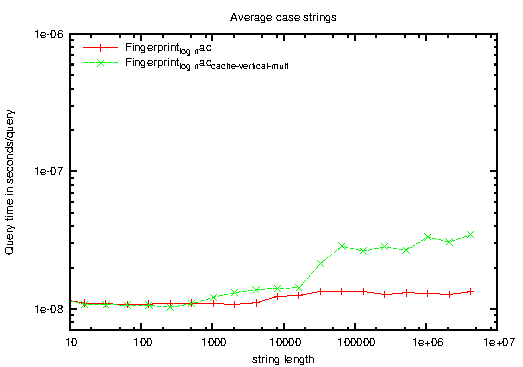
\includegraphics[width=0.49\textwidth,type=pdf,ext=.pdf,read=.pdf]{../src/results/length-fingerprint-log-cache-rand10.plt}
        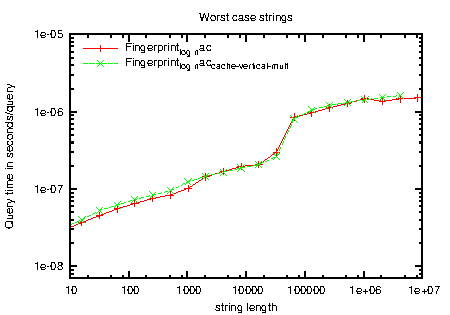
\includegraphics[width=0.49\textwidth,type=pdf,ext=.pdf,read=.pdf]{../src/results/length-fingerprint-log-cache-alla.plt}
    \end{center}
    \caption{\label{fig:plot-fingerprint-cache-vert}Query times of \fprint[2] with and without cache optimization.}
\end{figure}

\paragraph{Vertical, inter-level optimization}

\pref{fig:plot-fingerprint-cache-vert} shows results of our inter-level cache optimization. We see no improvement on worst case strings, and we see increased query times on average case strings. We conclude that this attempt at cache optimization does not improve practical query times, which could be expected, since it does not improve the asymptotic I/O bound either.

%%%%%%%%%%%%%%%%%%%%%%%%%%%%%%%%%%%%%%%%%%%%%%%%%%%%%%%%%%%%%%%%%%%%%%%%%%%%%%%
\subsection{Conclusions on Experimental Results}

Of the existing best \proc{DirectComp} and \proc{LcpRmq} algorithms, we have seen that \proc{DirectComp} is best on average case strings, while \proc{LcpRmq} is best on worst case strings.

We have found that our new \proc{DirectCompLookup} algorithm can improve the worst case query time performance of \proc{DirectComp}, while it does not degrade the average case query time to the level of \proc{LcpRmq}. However it is not as interesting as our new \fprintk\ algorithm, because it uses too much space.

Our new \fprintk\ algorithm is able to achieve a balance between worst case and average case query times. It has almost as good average case query times as \proc{DirectComp}, its worst case query times are significantly better than those of \proc{DirectComp}, and we have found cases between average and worst case where \fprintk\ is better than both \proc{DirectComp} and \proc{LcpRmq}. \fprintk\ gives a good time space tradeoff, and it uses less space than \proc{LcpRmq} when $k$ is small. The performance of \fprintk\ can be tweaked on many parameters, and we have found that optimizing for average case queries and for memory caches improve practical query time performance.

%%%%%%%%%%%%%%%%%%%%%%%%%%%%%%%%%%%%%%%%%%%%%%%%%%%%%%%%%%%%%%%%%%%%%%%%%%%%%%%
\subsection{Test Code}

To test practical performance, we have implemented the algorithms in C++. The implementation is based on that of Ilie~et~al.~\cite{ilie-navarro-tinta}, which we have heavily modified. We have made it compile on a 32-bit Windows architecture, and generalized it to allow more algorithms and tests to be implemented. \pref{tab:test-variables} summarizes the structure of the code and the parameters we can vary.

\begin{table}[tp]
\centering
\begin{tabular}{l l l}
Variable & Example & Component \\ \hline
alphabet size & $\sigma = 10$ & string \\
character pattern & uniformly at random & string \\ \hline
algorithm & \fprintk & algorithm \\
alg. parameter & $t = 2\sqrt n$ & algorithm \\ \hline
string length & exponentially increasing from $1$ to $100.000$ & test \\
query pattern & uniformly at random & test \\ \hline
\end{tabular}
\caption{List of performance variables tested.}\label{tab:test-variables}
\end{table}

In our implementation, we have made the following assumptions about the LCE problem:
\begin{itemize}
\item A character in a string is always eight bits.
\item A string always ends with a special null character, which does not occur anywhere else in the string. This does not affect our results, since we do not measure practical preprocessing time. If an algorithm has faster query times when the string ends in a special character, it could just add that character to the end of the string in its preprocessing.
\item We make no assumptions on the order of $i$ and $j$. In some applications of the LCE problem, for example approximate string searching, we know that $i<j$, and some algorithms might be able to take advantage of this knowledge to get faster query times. We do not measure this case.
\item Whenever we use random characters or query pairs, we use the \texttt{rand()} function from C. This gives repeatable pseudo-random numbers, which makes it easier for us to compare test runs.
\end{itemize}

% TODO \fixme{Results: Test Code: tell about c++ bug hunting in tinta, cachegrind code "Cache set count is not a power of two."}

%%%%%%%%%%%%%%%%%%%%%%%%%%%%%%%%%%%%%%%%%%%%%%%%%%%%%%%%%%%%%%%%%%%%%%%%%%%%%%%
\subsubsection{Query time by LCE value}

\begin{figure}[tp]
    \begin{center}
        %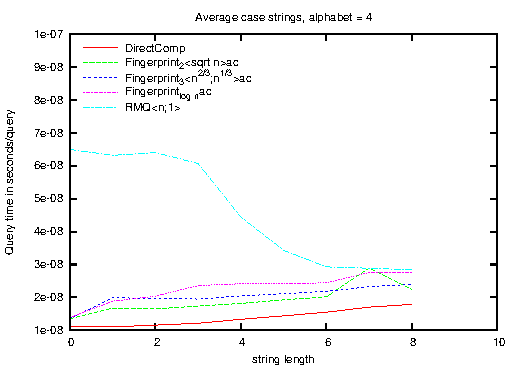
\includegraphics[width=0.49\textwidth,type=pdf,ext=.pdf,read=.pdf]{../src/results/value-article-rand4.plt}
        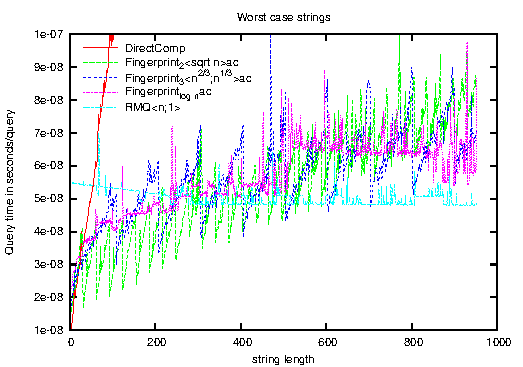
\includegraphics[width=0.49\textwidth,type=pdf,ext=.pdf,read=.pdf]{../src/results/value-article-alla.plt}
        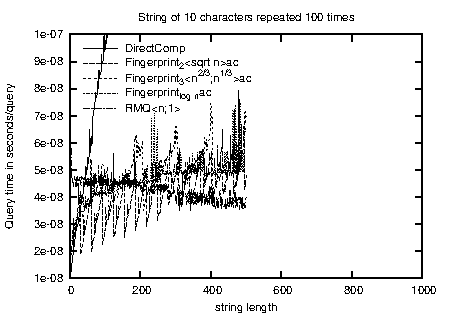
\includegraphics[width=0.49\textwidth,type=pdf,ext=.pdf,read=.pdf]{../src/results/value-article-repeat10-10.plt}
    \end{center}
    \caption{\label{fig:plot-by-value}Query times of some of our tested algorithms as a function of the returned LCE value.}
\end{figure}

As an alternative way of testing our algorithms, we have looked at how long a query takes in relation to the LCE value it returns, since most of our algorithms have query times, which depend on the returned LCE value. \pref{fig:plot-by-value} shows query times for a fixed string of 1000 characters. We can see how the query times of \fprint[2] and \fprint[3] increases as the LCE value increases, and drops when the LCE value becomes long enough to make one more step at the higher level with fingerprints of longer substrings. We also see that the query time of \fprint[\log n] increases whenever the LCE value becomes long enough to reach a higher level of the data structure.

The plots in \pref{fig:plot-by-value} contains a lot of noise compared to our other plots. The number of measurements we make on these plots is many times bigger than the number of measurements we make on other plots. Therefore each measurement is an average over only 10000 queries instead of a million queries, which gives less accurate results.

We need to measure a sum of many queries to get an accurate timing, since each individual query is too fast to measure. While measuring a sequence of randomly generated queries is a very artificial test, which is unlikely to occur in practice, we think that it is even more artificial to measure a sequence of queries for which we already know that the LCE value is the same each time. On our worst case string $s=aaaaaaa...$, the queries we measure in each point in \pref{fig:plot-by-value} have the pattern $\max(i,j)=v$, which may give very different performance characteristics compared to random queries due to cache effects. We cannot meaningfully measure performance by LCE value on average case strings, as these strings do not contain large LCE values. The second plot in \pref{fig:plot-by-value} is on a string, which attempts to avoid a strong pattern like $\max(i,j)=v$ while it still has large LCE values.

Because of the amount of noise in the plots and the strong pattern of $\max(i,j)=v$, we have not focused on this way of measuring query time performance in our analysis.

\begin{comment}
\begin{algorithm}
\caption{Algorithm for plotting query time as a function of string length\label{alg:graph-length}}
\begin{codebox}
\li \For $\id{type} \in \{\textrm{string of random characters with}~\sigma=10,~\textrm{string with}~\sigma = 1\}$
    \Indentmore
\li     \For $n = 1$ \To $1e7$ \Comment Double $n$ at each iteration
        \Indentmore
\li         $s = \proc{MakeString}_{\id{type}}(n)$
\li         $\id{data} =$ a sequence of a million pairs $(i,j)$ where
            \Indentmore
\zi             $i\in[1\twodots n]$ and $j\in[1\twodots n]$ are chosen
\zi             uniformly at random.
            \End
\li         \For each $\id{alg} \in \id{Algorithms}$
            \Indentmore
\li             $\id{alg}.\proc{preprocess}(s)$
\li             start timing
\li             \For each $(i,j) \in \id{data}$
                \Indentmore
\li                 $\id{alg}.\proc{query}(i,j)$
                \End
\li             end timing
\li             \proc{Plot}$_{\id{type}}$($alg$, $n$, timing)
\li             $\id{alg}.\proc{cleanup}()$
            \End
        \End
    \End
\end{codebox}
\end{algorithm}

\begin{algorithm}
\caption{Algorithm for plotting query time as a function of LCE value\label{alg:graph-value}}
\begin{codebox}
\li $s = \proc{MakeString}(1000)$
\li \id{data} = an array where $\id{data}[v] \subseteq \{(i,j)~|~\LCE(i,j)=v\} \land |\id{data}[v]| =10.000$
\li \For each $\id{alg} \in \id{Algorithms}$
    \Indentmore
\li     $\id{alg}.\proc{preprocess}(s)$
\li     \For $v = 0$ \To $n$
        \Indentmore
\li         \Repeat 3 times
% \li     $A =$ generate 1000000 random pairs $(i,j)$ where $i<j$
\li             start timing
\li             \For each $(i,j) \in data[v]$
                \Indentmore
\li                 $\id{alg}.\proc{query}(i,j)$
                \End
\li             end timing
            \End
\li         \proc{Plot}($alg$, $v$, median of the three timings)
        \End
\li     $\id{alg}.\proc{cleanup}()$
    \End
\end{codebox}
\end{algorithm}

Where $\proc{Plot}(f,x,y)$ adds point $(x,y)$ to series $f$.
\end{comment}

%%%%%%%%%%%%%%%%%%%%%%%%%%%%%%%%%%%%%%%%%%%%%%%%%%%%%%%%%%%%%%%%%%%%%%%%%%%%%%%
%%%%%%%%%%%%%%%%%%%%%%%%%%%%%%%%%%%%%%%%%%%%%%%%%%%%%%%%%%%%%%%%%%%%%%%%%%%%%%%
\section{Ziv-Lempel Compression\label{sec:lz-compress}}

\newcommand{\zreference}{\textit{reference}}
\newcommand{\zlabel}{\textit{label}}
\newcommand{\zphrase}{\textit{phrase}}

Sometimes it can be useful to store a string in a compressed format and query the compressed string directly without using extra space and time to first decompress the string. In this section we explore the LCE problem on strings compressed using LZ78 compression. We look at solutions, which require space proportional to the compressed size of a string, and are able to answer LCE queries fast.

%%%%%%%%%%%%%%%%%%%%%%%%%%%%%%%%%%%%%%%%%%%%%%%%%%%%%%%%%%%%%%%%%%%%%%%%%%%%%%%
\subsection{LZ78 definition\label{sec:lz-definition}}
A string $s$ of length $N$ has a corresponding \textit{compressed string} $z$ of compressed length $n$, where $z$ is a list of \textit{compression elements}, $z = z_1, z_2, ..., z_n$. Each compression element $z_x$ is a pair $(r_x, \alpha_x)$, where the reference, $\zreference_z(x)=r_x$, is an index of an earlier compression element in the compressed string or zero, i.e. $0 \leq \zreference_z(x) < x$, and the label, $\zlabel_z(x)=\alpha_z$, is a character from the original uncompressed string $s$. The \zphrase\ of a compression element is defined as:
\begin{align*}
\zphrase_z(x) =
\begin{cases}
    \zphrase_z(\zreference_z(x)) \cdot \zlabel_z(x) & \textrm{if}~ \zreference \neq 0\\
    \zlabel_z(x) & \textrm{otherwise}
\end{cases}
\end{align*}
where "$\cdot$" denotes string concatenation. From a compressed string $z = z_1,...,z_n$, we can get the original string $s=\zphrase_z(1)\cdot...\cdot\zphrase_z(n)$.

We can easily get the decompressed string $s$ from the compressed string $z$ using the definitions. To get the compressed string $z$ from the original string $s$ we can look at the compression elements as a tree, where the reference of each compression element corresponds to the parent pointer of each node in the tree. We consume $s$ from left to right while we build the tree:
\begin{enumerate}
\item Let the tree be single special root node $z_0$, let $i = 1$ and $c=z_0$.
\item If $c$ has a child $u$, where $\zlabel(u)=s[i]$, set $c=u$. Otherwise create the child node $u$, set $\zlabel(u)=s[i]$ and set $c=z_0$.
\item Increment $i$ by one and repeat from step 2 until the entire string is consumed when $i = n$.
\end{enumerate}
The compressed string $z$ is now the tree except the special root node $z_0$.

The size of the compressed string is at most $n=O(N)$ and at least $n=\Omega(\sqrt{N})$.
% N= 1+2+3+4+...+n=(n^2+n)/2

%%%%%%%%%%%%%%%%%%%%%%%%%%%%%%%%%%%%%%%%%%%%%%%%%%%%%%%%%%%%%%%%%%%%%%%%%%%%%%%
\subsection{Compressed \proc{DirectComp}\label{sec:lz-iterate-forward}}

We can adapt \proc{DirectComp} to work on a compressed string. To work directly on a compressed string, we first need to have random access to the characters of the original string.

\begin{lemma}
\label{lem:lz-random-access}
Let $s$ be a string of length $N$ and let $z$ of length $n$ be the LZ-compression of $s$. For any $1 \leq i \leq N$, we can find $s[i]$ in $O(\log\log N)$ query time using $O(n)$ space.
\end{lemma}

\begin{proof}
To find the character $s[i]$, we can first use a Predecessor query to find out which compression element $s[i]$ is in. We can then use a Level Ancestor query to find the correct character from the found compression element.

% We can find the $i$'th character of $s$ as $s[i] = \zphrase(\proc{Pred}(i))[i - \textit{start}[\proc{Pred}(i)]]$ where $\proc{Pred}(i)$ is the index of the compression element containing $s[i]$, and $\textit{start}[x]$ is the position in $s$ of the first character of $\zphrase(x)$, i.e. $s[\textit{start}[x]] = \zphrase(x)[1]$.

% We can find \proc{Pred}(i) with a predecessor query over predecessor datastructure of the $n$ compression elemets, where each compression element $x$ is added using $\textit{start}[x] as its key, and the universe has size N. When we look at the compression elements as a tree, we have $\zlabel(x)[i]=\proc{Level-Ancestor}(i,x)$. We therefore have random access to che characters of a compressed string using one Predecessor query and one Level Ancestor query.

The query time for a random access query is $O(\log\log N)$, since we use $O(\log\log N)$ time on the Predecessor query and $O(1)$ time on the Level-Ancestor query. The space needed to support random access queries is $O(n)$, since both the predecessor data structure and the level ancestor data structure use $O(n)$ space.
\end{proof}

\begin{theorem}
Let $s$ be a string of length $N$ and let $z$ of length $n$ be the LZ-compression of $s$. Compressed \proc{DirectComp} can find $\LCE(i,j)$ in $O(\log\log N + |\LCE(i,j)|)$ query time using $O(n)$ space.
\end{theorem}

\begin{proof}
Whenever \proc{DirectComp} reads a character of the string $s$, we instead use the random access described in \pref{lem:lz-random-access} to read the character from the compressed string. The predecessor query is only needed in the first comparison of the two indexes $i$ and $j$ in $\LCE(i,j)$. In subsequent iterations of \proc{DirectComp} we know that we always need the same compression element or the following compression element as we used in the previous iteration of the loop, and we therefore do not need the predecessor query to find the compression element. The total query time for \proc{DirectComp} on LZ-compressed strings becomes $O(\log\log N + |\LCE(i,j)|)$, which is $O(N)$ in worst case and $O(\log \log N)$ on average.
\end{proof}

%%%%%%%%%%%%%%%%%%%%%%%%%%%%%%%%%%%%%%%%%%%%%%%%%%%%%%%%%%%%%%%%%%%%%%%%%%%%%%%
\subsection{Reversed Compressed \proc{DirectComp}}

A simpler way of doing LCE on compressed a string is to reverse the string and then run \proc{DirectComp} in the reverse direction on the reversed string, which gives the same result since reversing a string twice gives the original string. Where \proc{DirectComp} compares $s[i+v]$ against $s[j+v]$ in each iteration of its loop, reversed \proc{DirectComp} compares $s[N+1-i-v]$ against $s[N+1-j-v]$ in each iteration. This is simpler than using \proc{DirectComp} directly on the compressed string, because Level Ancestor queries are no longer needed at each iteration, since we can use the reference of the current compression element as follows, where the position of each of $i$ and $j$ is stored as a pair $(x,y)$:
\begin{align*}
\proc{PreviousPosition}(x, y)=&
\begin{cases}
(\zreference(x), y) & \textrm{if} ~ \zreference(x) \neq 0 \\
(y-1, y-1) & \textrm{if} ~ y > 1\\
\textit{End of string} & \textrm{otherwise}
\end{cases}\\
\proc{Character}(x, y)=&~\zlabel(x)\\
\proc{Position}(i)=&~(x,y)~\textrm{where}\\
&~~y=\proc{Predecessor}(i)~\textrm{and}\\
&~~x=\proc{Level-Ancestor}(i-\proc{Start-Of}(y), y)
\end{align*}
We then only need one Predecessor and one Level Ancestor query to initialize each of the two pairs.

%%%%%%%%%%%%%%%%%%%%%%%%%%%%%%%%%%%%%%%%%%%%%%%%%%%%%%%%%%%%%%%%%%%%%%%%%%%%%%%
\subsubsection{Random Access Initialization}

We can try to completely avoid Predecessor and Level Ancestor when initializing the pair $(x,y)$. We could try to store all $N$ pairs, but that would require $O(N)$ space and defeat the purpose of compression. We could also just walk from the end of the string to the desired position, but that would bring the average case query time up to $O(N)$. Similarly to how \proc{DirectCompLookup} works, we can store some of these positions. If we store $t$ positions equally spaced across the string $s$, we would get $O(n+t)$ space and $O(N/t+|\LCE(i,j)|)$ query time. To keep the compressed space, we can set $t=n$, which gives $O(N/n+|\LCE(i,j)|) = O(\sqrt{N}+|\LCE(i,j)|)$ query time. 

%%%%%%%%%%%%%%%%%%%%%%%%%%%%%%%%%%%%%%%%%%%%%%%%%%%%%%%%%%%%%%%%%%%%%%%%%%%%%%%
\subsubsection{Length of the Reversed String}

Reversing the string can be done in $O(N)$ time and $O(n_1 + n_2)$ space, where $n_1$ and $n_2$ are the compressed lengths of the original and reversed string respectively. To achieve this, we have already shown how we can read a string from right to left one character at a time in $O(1)$ space, and the compression algorithm described in \pref{sec:lz-definition} reads its input string one character at a time from left to right and uses $O(n)$ space for its tree of compression elements.

But the question is how big $n_2$ is relative to $n_1$. From knowing how much compression is possible with LZ-compression, we can see that $n_2=O(n_1^{~2})$. It might be possible to improve that bound, but for the string $z=(0,a)$ $(1,b)$ $(2,c)$ $...$ $(n-1,z)$, we have experimentally determined that reversing $z$ gives $n_2=0.89n_1^{~1.51}$, so we cannot get an optimal bound of $n_2=O(n_1)$. This is a disadvantage of doing LCE on the reversed string compared to doing it on the original compressed string using Level Ancestor queries.

%%%%%%%%%%%%%%%%%%%%%%%%%%%%%%%%%%%%%%%%%%%%%%%%%%%%%%%%%%%%%%%%%%%%%%%%%%%%%%%
\subsection{Using Compression to Speed Up \proc{DirectComp}}

Our original goal of looking into compression was to see if using the techniques used in compression could improve the worst case query time of \proc{DirectComp} to something better than $O(N)$. Our idea is that whenever you have a long LCE value, you have a repetition within the string, and repetitions would typically give good compression. If the compressed string can be searched over similarly to how \proc{DirectComp} searches the uncompressed string, it might be possible to establish a better worst case query time.

We have found one case where we can make compressed \proc{DirectComp} faster than \proc{DirectComp} on uncompressed strings, but our finding does not improve worst case query time. We explain this in terms of the reversed compressed \proc{DirectComp}, as it is simpler, but it also works without the string reversal. Reversed compressed \proc{DirectComp} starts with two positions $(x_i,y_i)$ and $(x_j,y_j)$ corresponding to the two positions $i$ and $j$ in $\LCE(i,j)$. At each iteration, it then updates $(x_i,y_i)$ and $(x_j,y_j)$ to find the previous two positions. If $x_i = x_j$ we know that we can add $\textit{depth}[x_i]$ to the LCE value, where \textit{depth} is the depth of a node in the tree of compression elements. Compressed \proc{DirectComp} can then compare $\textit{depth}[x_i]$ characters in constant time.

Through this technique can improve query time in some cases, it does not improve the worst case time of $\Theta(N)$. This is because we cannot be sure to hit the condition allowing us to compare many characters in constant time, even for long LCE values. As an example, $LCE(1,2)$ on a string where all $N$ characters are the same takes $\Omega(N)$ time. For such a string, the tree representing the compressed string is always a path, and $x_i$ and $x_j$ will always be either a node and its parent or the root and some other node. They will therefore never end up being the same node at the same time, as shown in \pref{fig:lz-no-jumps}.

\begin{figure}[tp]
    \begin{center}
        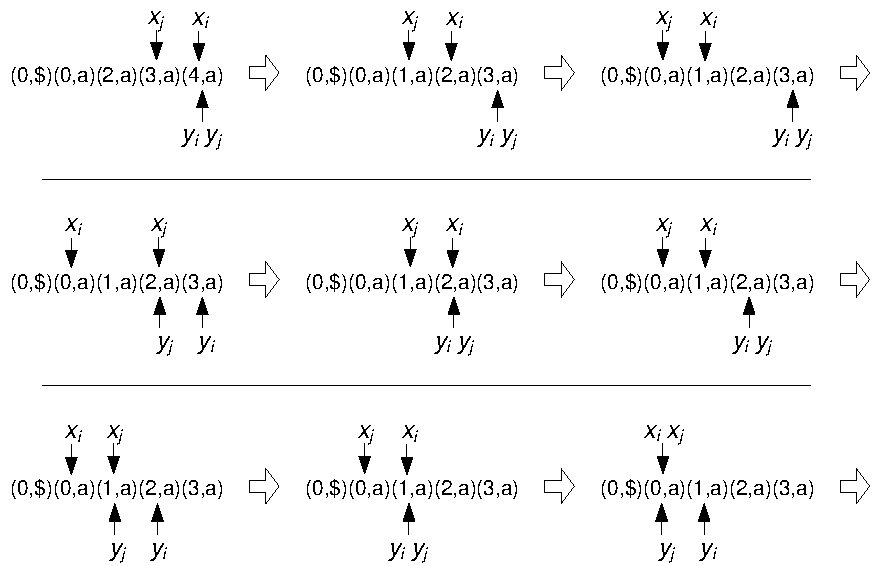
\includegraphics[width=0.9\textwidth]{lz.pdf}
    \end{center}
    \caption{\label{fig:lz-no-jumps}Reversed compressed \proc{DirectComp} for $LCE(1,2)$ on the string $s=aaaaaaaaaa\$$. None of the steps can be skipped, since $x_i$ and $x_j$ are never the same.}
\end{figure}

% \fixme{Compression: But can we cache some results as we go even if pointers are not the same? No, that is Theta(n**2) = Omega(N) space. But do we really need it all?}

%%%%%%%%%%%%%%%%%%%%%%%%%%%%%%%%%%%%%%%%%%%%%%%%%%%%%%%%%%%%%%%%%%%%%%%%%%%%%%%
\subsection{Compression with Other Algorithms\label{sec:lz-other}}

We can look at the other LCE algorithms we have examined in addition to \proc{DirectComp}, and see if we can apply them to LZ-compressed strings. We have not found a way to apply \proc{SuffixNca} or \proc{LcpRmq}, as the string we want to find LCE values on still has N suffixes, and we have not found a way to relate the compression rate of the NCA structure or suffix array to the compression rate of the string.

Fingerprinting does not compress well either. We could LC-compress each level of fingerprints just like the original string is compressed, but as the substrings fingerprinted becomes longer at each elvel, the compression ration becomes worse, and at the top level with $t_\ell = \Omega(N)$, we need $\Omega(N)$ space to store $H_\ell$, since all fingerprints would be unique or have very few copies.

Since we have not been able to find improvements to the $O(N)$ worst case query time in $O(n)$ space using existing algorithms, we have looked into new algorithms. The compression elements of a compressed string $z$ forms a tree, and each phrase in $z$ is a path in the tree. The LCE value is the length of a substring, which occurs at two positions $i$ and $j$ in the input string. This substring spans a number of phrases, where each phrase is a path in the tree of compression elements. If we can make fast LCE queries on such a tree, we can make fast LCE queries on highly compressable strings.

\begin{theorem}
\label{thm:lz-tree}
Let $s$ be a string of length $N$ and let $z$ of length $n$ be the LZ-compression of $s$. We can preprocess $z$ using $O(n)$ space to answer LCE queries $v=\LCE(i,j)$ in $O(\log\log N + \log n \cdot \textit{\#phrases})$ time, where \textit{\#phrases} is the number of phrases of $z$ used to store $s[i\twodots i+v]$ and $s[j\twodots j+v]$.
\end{theorem}

\begin{proof}
In \pref{sec:tree-lce} we describe how to perform LCE queries on a static tree of $n$ nodes in $O(\log n)$ query time and $O(n)$ space. We can first find the positions of $i$ and $j$ within $z$ in $O(\log\log N)$ time, and then we can repeat the $O(\log n)$ tree LCE query \textit{\#phrases} times to find the LCE value.
\end{proof}

%%%%%%%%%%%%%%%%%%%%%%%%%%%%%%%%%%%%%%%%%%%%%%%%%%%%%%%%%%%%%%%%%%%%%%%%%%%%%%%
\subsection{Cache Performance}

We have looked into the cache performance of compressed \proc{DirectComp}. If the string does not compress at all, i.e.\ the compressed string is $z=(0,a)(0,b)(0,c)...$, \proc{DirectComp} reads from the string in the best way possible using $O(N/B)$ I/O's in worst case. When the string is LZ-compressable, the I/O pattern becomes much worse. If $\zreference(x_1) = x_2 > 0$, the algorithm will read from position $x_1$ and then $x_2$, and these two may not be next to each other in memory. This can happen many times, which gives $O(N)$ I/O's in worst case.

We could lay out the tree of compression elements in memory as a B-tree, where we store groups of adjacent nodes next to each other in memory, to optimize the number of I/O's within each phrase, but each node may have more than $B$ children, and in this case it would not improve the worst case number of I/O's, as each node visited may be in a new group.

%%%%%%%%%%%%%%%%%%%%%%%%%%%%%%%%%%%%%%%%%%%%%%%%%%%%%%%%%%%%%%%%%%%%%%%%%%%%%%%
%%%%%%%%%%%%%%%%%%%%%%%%%%%%%%%%%%%%%%%%%%%%%%%%%%%%%%%%%%%%%%%%%%%%%%%%%%%%%%%
\section{LCE on Trees\label{sec:tree-lce}}

To achieve the result of \pref{thm:lz-tree}, we need to do LCE on a tree in $O(\log n)$ query time and $O(n)$ space. In this section we analyze ways to achieve this.

%%%%%%%%%%%%%%%%%%%%%%%%%%%%%%%%%%%%%%%%%%%%%%%%%%%%%%%%%%%%%%%%%%%%%%%%%%%%%%%
\subsection{Definition\label{sec:tree-def}}

Let $T$ be a rooted tree with $n$ nodes where each edge from parent node $p$ to child node $c$ is labeled with a character $\zlabel(c)$.
Let $p_i$ be a path in $T$ from a node $u_i$ to a node $w_i$, such that $w_i$ is a descendant of $u_i$, and
let $p_j$ be a path in $T$ from a node $u_j$ to a node $w_j$, such that $w_j$ is a descendant of $u_j$.
Then $\LCE_T(p_i, p_j)$ is the length of the longest common prefix of $s_i$ and $s_j$, where
$s_i$ is the concatenation of the edge labels of $p_i$, and
$s_j$ is the concatenation of the edge labels of $p_j$.

This definition of LCE on a tree is chosen to match the tree of LZ compression elements and the necessary LCE queries on it described in \pref{sec:lz-other}.

To simplify our description of our tree LCE algorithms, we define $p_i(v)$ to be the node on $p_i$ with distance $v$ to $u_i$, and similarly for $p_j(v)$. We can calculate $p_i$ in constant time as $p_i(v)=\LA(d(u_i)+v,w_i)$, where $d(u_i)$ is the depth of $u_i$, and $\LA$ is a Level Ancestor query.

%%%%%%%%%%%%%%%%%%%%%%%%%%%%%%%%%%%%%%%%%%%%%%%%%%%%%%%%%%%%%%%%%%%%%%%%%%%%%%%
\subsection{Walking the Paths with Level Ancestor\label{sec:tree-dc}}

We can find $\LCE(i,j)$ in $O(|\LCE(i,j)|)$ query time using Level Ancestor, in the same way \proc{DirectComp} finds LCE on strings: First compare $\textit{label}(p_i(1))$ to $\textit{label}(p_j(1))$, then compare $\textit{label}(p_i(2))$ to $\textit{label}(p_j(2))$ and so on until the two characters differ or either $w_i$ or $w_j$ is reached.

\begin{theorem}
\proc{TreeDirectComp} can preprocess a static tree of $n$ nodes to answer LCE queries as defined in \pref{sec:tree-def} using $O(|\LCE(i,j)|)$ query time, and $O(n)$ space and preprocessing time.
\end{theorem}
\begin{proof}
Each Level Ancestor query takes constant time, and we do $2|\LCE(i,j)| + 2$ of them, giving us $O(|\LCE(i,j)|)$ query time. The space and preprocessing requirement of Level Ancestor is $O(n)$.
\end{proof}

%%%%%%%%%%%%%%%%%%%%%%%%%%%%%%%%%%%%%%%%%%%%%%%%%%%%%%%%%%%%%%%%%%%%%%%%%%%%%%%
\subsection{Using Fingerprinting}

\newcommand{\tfprint}[1][k]{\ensuremath{\proc{TreeFingerprint}_{#1}}}
\newcommand{\tfprintk}{\tfprint[k]}

We can adapt our \fprintk\ algorithm on strings to work on trees, which we call \tfprintk. If we store the fingerprint of $s[i\twodots i+t_\ell]$ in $H_\ell[i+t_\ell]$ instead of $H_\ell[i]$, then the \fprintk\ query directly adapts to \tfprintk. If we wanted to use the same preprocessing as we use for \fprintk\ on strings, we would have to adapt the suffix array to apply to trees, and find a way to construct it in $\sortt$ time, which we have not looked at. Instead we can preprocess the fingerprints of the tree with Karp-Miller-Rosenberg~\cite{karp-miller-rosenberg}.

\begin{theorem}
\tfprintk, where $k$ is a parameter $1\leq k\leq\logceil$, can preprocess a static tree of $n$ nodes to answer LCE queries as defined in \pref{sec:tree-def} using $O(k\cdot n^{1/k})$ query time, $O(k\cdot n)$ space, and $O(n\log n)$ preprocessing time.
\end{theorem}

\subsubsection{Data Structure}

We define a natural number $F_t[u]$ to be the fingerprint for node $u$ of length $t$. For two nodes $u$ and $w$ in a tree $T$, their fingerprints $F_t[u]$ and $F_t[w]$ of the same length $t$ are the same if and only if the last $t$ characters on the path from the root of $T$ to $u$ is the same as the last $t$ characters on the path from the root of $T$ to $w$.

For a given parameter $k$, where $1\leq k \leq \logceil$, we define the \tfprintk\ data structure as follows: For each number $\ell$ between $0$ and $k-1$, let $t_\ell=\Theta(n^{\ell/k})$, and let $t_0 = 1$. For each number $\ell$ between $0$ and $k-1$ and each node $u$ in $T$, whose depth is at least $t_\ell$, let $H_\ell[u] = F_{t_\ell}[u]$

\begin{lemma}
The \tfprintk\ data structure takes $O(k\cdot n)$ space.
\end{lemma}
\begin{proof}
The data structure contains $k$ numbers $t_\ell$ and $k$ tables of fingerprints $H_\ell$, and each table contains fingerprints for at most all of the $n$ nodes in the tree.
\end{proof}

\subsubsection{Query}

The quey for \tfprintk\ is nearly the same as the query for \fprintk\ on strings, except we replace $H_\ell[i+v]$ and $H_\ell[j+v]$ with $H_\ell[p_i(v+t_\ell)]$ and $H_\ell[p_j(v+t_\ell)]$. We also stop the algorithm after we reach $p_i(v+t_\ell)=w_i$ or $p_j(v+t_\ell)=w_j$.

\begin{lemma}
The \tfprintk\ query finds the correct tree LCE value in $O(k\cdot n^{1/k})$ time.
\end{lemma}
\begin{proof}
We have changed nothing from the \fprintk\ query on strings, which negatively affects the query time, so the query time is the same.

% The combination of Level Ancestor and the definition that a fingerprint relates to a substring from a given node to an ancestor that node, ensures that the fingerprints we choose to compare are the fingerprints, which represents the strings on the paths from $u_i$ to $w_i$ and from $u_j$ to $w_j$.

\begin{figure}[tp]
    \begin{center}
        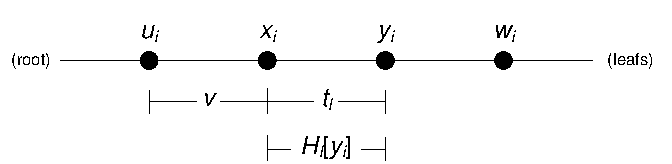
\includegraphics[width=0.7\textwidth,page=1]{tree-fingerprint.pdf}
    \end{center}
    \caption{\label{fig:tree-query}Finding the right fingerprint to look at for a \tfprintk\ query.}
\end{figure}

The fingerprints we choose to compare are the fingerprints, which represents substrings on $p_i$ and $p_j$. At any given iteration at level $\ell$, the query algorithm has already looked at the string on the path from $u_i$ to $p_i(v)$, and we now need to look at the string on the path from $p_i(v)$ to $p_i(v+t_\ell)$, as shown in \pref{fig:tree-query}. From our definition of fingerprints in a tree, this string has fingerprint $H_\ell[p_i(v+t_\ell)]$. The LCE query is therefore correct when we use $H_\ell[p_i(v+t_\ell)]$ (and similar for $j$ instead of $i$).
\end{proof}

\subsubsection{Preprocessing}

We use Karp-Miller-Rosenberg~\cite{karp-miller-rosenberg} to preprocess the \tfprintk\ data structure. When $t_\ell$ is $t_{\ell-1} < t_\ell \leq 2t_{\ell-1}$, we preprocess level $\ell$ like this:
\begin{enumerate}
\item Make pairs of fingerprints $H_\ell[u] = (H_{\ell-1}[LA(d(u)-t_\ell+t_{\ell-1},u)], H_{\ell-1}[u])$ for all $u$ where $d(u) \geq t_\ell$.
\item Sort the pairs lexicographically.
\item Replace each pair with a new fingerprint, by going through them in lexicographical order, while updating the fingerprint whenever the pair changes.
\end{enumerate}

Repeat the steps above for each level, starting with $\ell = 1$ and ending with $\ell = k-1$. When $k < \logceil$, the condition that $t_\ell \leq 2t_{\ell-1}$ is not satisfied. In this case we need to add extra levels in the preprocessing, which we will only store temporarily. We therefore always need to preprocess $O(\log n)$ levels, even if we only store some of them.

\begin{lemma}
The KMR algorithm for preprocessing \tfprintk\ gives the correct data structure.
\end{lemma}
\begin{proof}
Two strings $S$ and $T$ of length $a$ are the same if and only if we can split each of them into two smaller substrings $S = S_1\cdot S_2$ and $T=T_1\cdot T_2$ such that $S_1=T_1$ and $S_2=T_2$, where "$\cdot$" is string concatenation. Therefore we can assign fingerprints $F_a[S]=F_b[S_1]\cdot F_c[S_2]$ and $F_a[T]=F_b[T_1]\cdot F_c[T_2]$ in step one of the preprocessing algorithm. The same also holds when the two smaller substrings overlap.

The fingerprints from level $\ell-1$ are natural numbers, less than $n$. Step one of the preprocessing algorithm makes each fingerprint at level $\ell$ a natural number less than $n^2$. Step two and three of the preprocessing algorithm reduces that universe of fingerprints back to $n$ without changing the equality of the fingerprints.
\end{proof}

\begin{lemma}
The KMR algorithm for preprocessing \tfprintk\ takes $O(n\log n)$ time.
\end{lemma}
\begin{proof}
Step one and three use linear time. In step two we can use radix sort, which uses linear time, because our universe of elements to sort is $n^2$. The total preprocessing time becomes $O(n\log n)$ for preprocessing $\log n$ levels in $O(n)$ time each.
\end{proof}

%%%%%%%%%%%%%%%%%%%%%%%%%%%%%%%%%%%%%%%%%%%%%%%%%%%%%%%%%%%%%%%%%%%%%%%%%%%%%%%
\subsection{Using Constant Time String LCE in Heavy Paths}

To answer LCE queries on a tree, we can create a heavy path decomposition of the tree and create a string of the labels of all the heavy paths concatenated. We can then use constant time string LCE on this string. We call this algorithm \proc{HeavyPathLce}.

\begin{theorem}
\proc{HeavyPathLce} can preprocess a static tree of $n$ nodes to answer LCE queries as defined in \pref{sec:tree-def} using $O(\log n)$ query time, $O(n)$ space, and $O(\sortt)$ preprocessing time.
\end{theorem}

\subsubsection{Data Structure}

\begin{figure}[tp]
    \begin{center}
        \includegraphics[width=0.5\textwidth,page=4]{tree-fingerprint.pdf}
    \end{center}
    \caption{\label{fig:tree-heavy-ds}A heavy path decomposition of a tree and a corresponding \proc{HeavyPathLce} string $s$.}
\end{figure}

The \proc{HeavyPathLce} data structure consists of the following:
\begin{itemize}
\item An input tree $T$ with a heavy path decomposition.
\item A string $s$, which is a concatenation of all heavy path labels of $T$, where the label of a heavy path is the concatenation of the label on a light edge, and the labels on all edges on the heavy path following that light edge. \pref{fig:tree-heavy-ds} shows an example of $s$.
\item For a node $u$, $\textit{end}(u)$ points to the node of greatest depth in $u$'s heavy path, $d(u)$ is the depth of $u$, and $\textit{index}(u)$ is the index in $s$, which stores $\zlabel(u)$.
\item Data structures for constant time NCA on $T$, constant time LA on $T$, and constant time LCE on $s$.
\end{itemize}

\begin{lemma}
The \proc{HeavyPathLce} data structure takes $O(n)$ space.
\end{lemma}
\begin{proof}
The string $s$ contains $n-1$ characters, one for each edge in $T$. The space usage for NCA, LA, LCE, and the extra information about each node (\textit{end}, \textit{index}, and \textit{d}) is all $O(n)$.
\end{proof}

\begin{lemma}
We can preprocess the \proc{HeavyPathLce} data structure in $O(\sortt)$ time.
\end{lemma}
\begin{proof}
Preprocessing LCE on $s$ using \proc{SuffixNca} or \proc{LcpRmq} takes $O(\sortt)$ time. If we walk through the tree and for each leaf append the heavy path ending in that leaf to $s$, we can construct $s$ in $O(n)$ time. The rest of the data structures can be preprocessed in $O(n)$ time.
\end{proof}

\subsubsection{Query}

In a \proc{HeavyPathLce} query $\LCE_T(p_i,p_j)$ we start with $v=0$ and do the following repeatedly:
\begin{enumerate}
\item Stop when we reach either $p_i(v)=w_i$ or $p_j(v)=w_j$, and return $v$.
\item Find $v'=\LCE_s(\textit{index}(p_i(v+1)),\textit{index}(p_j(v+1)))$.
\item Find $m_i = d(\NCA_T(\textit{end}(p_i(v+1)), w_i))-(d(u_i)+v)$.
\item Find $m_j = d(\NCA_T(\textit{end}(p_j(v+1)), w_j))-(d(u_j)+v)$.
\item Stop if $v'<\min(m_i,m_j)$ and return $v+v'$.
\item Otherwise increment $v$ by $\min(m_i,m_j)$.
\end{enumerate}

\begin{lemma}
The \proc{HeavyPathLce} query finds the correct LCE value.
\end{lemma}
\begin{proof}
The query algorithm maintains the invariant $v\leq\LCE_T(p_i,p_j)$. In step three, $m_i$ is the number of edges on a single heavy path at the beginning of the path from $p_i(v)$ to $w_i$, and similar for $m_j$ in step four, like illustrated in \pref{fig:tree-heavy-query}. The labels of these edges are stored consecutively in $s$. If $v'<\min(m_i,m_j)$, the LCE query found the longest common prefix to be within both of the two paths $p_i$ and $p_j$ we are searching, and we have therefore found the LCE value and stop. If $v'\geq\min(m_i,m_j)$, we had a matching prefix which was as long or longer than the part of the heavy path we are interested in, and we therefore need to continue looking at the next heavy path to find the LCE value.

\begin{figure}[tp]
    \begin{center}
        \includegraphics[width=0.7\textwidth,page=2]{tree-fingerprint.pdf}
    \end{center}
    \caption{\label{fig:tree-heavy-query}How we find $m_i$ and $m_j$ in a \proc{HeavyPathLce} query.}
\end{figure}
\end{proof}

\begin{figure}[tp]
    \begin{center}
        \includegraphics[width=0.25\textwidth,page=3]{tree-fingerprint.pdf}
    \end{center}
    \caption{\label{fig:tree-heavy-query2}A \proc{HeavyPathLce} query with at most five iterations. Heavy edges on $p_i$ and $p_j$ are marked bold.}
\end{figure}

\begin{lemma}
The \proc{HeavyPathLce} query takes $O(\log n)$ time.
\end{lemma}
\begin{proof}
Since there is at most $O(\log n)$ light edges in any simple path in $T$, the two paths $p_i$ and $p_j$ contains at most $O(\log n)$ light edges in total. Since and each iteration of the query takes constant time, and we reach reach a new light edge in each iteration, as shown in \pref{fig:tree-heavy-query2}, the query time is $O(\log n)$.
\end{proof}

\begin{comment}
LCE(u_i,w_i,u_j,w_j)
    v_i = u_i
    v_j = u_j
    v = 0
    while v_i != w_i && v_j != w_j
        Let m_i be the number of initial heavy edges on the path from v_i to w_i before any light edge.
        Let m_j be ...
        //m_i and m_j can be calculated in constant time.
        Let m = min(m_i, m_j)
        if m = 0
            if the two next characters are the same
                advance one character
            else
                stop
        else
            v=LCE_s(index(v_i),index(v_j))
            If v >= m
                advance m characters using Level Ancestor
            else
                advance v characters
                stop

    O(log n) time, one step for each light edge encountered on each of the two paths.
\end{comment}

%%%%%%%%%%%%%%%%%%%%%%%%%%%%%%%%%%%%%%%%%%%%%%%%%%%%%%%%%%%%%%%%%%%%%%%%%%%%%%%
\subsection{Directly Mapping \proc{SuffixNca} and \proc{LcpRmq}}

\begin{figure}[tp]
    \begin{center}
        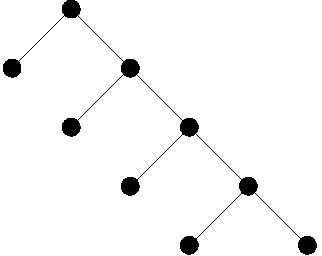
\includegraphics[width=0.25\textwidth]{quadratic-tree.pdf}
    \end{center}
    \caption{\label{fig:quadratic-tree}A tree with $\Omega(n^2)$ ways to choose a leaf and an ancestor of that leaf.}
\end{figure}

We have looked at applying \proc{SuffixNca} and \proc{LcpRmq} directly to trees like we did with \proc{DirectComp} and \fprintk, such that we can get $O(1)$ query time.

\begin{theorem}
\proc{TreeLcpRmq} and \proc{TreeSuffixNca} can preprocess a static tree of $n$ nodes to answer LCE queries as defined in \pref{sec:tree-def} using $O(1)$ query time and $O(n^2)$ space.
\end{theorem}
\begin{proof}
\proc{LcpRmq} relies on accessing two suffixes in SA, $i$ and $j$. In \proc{TreeLcpRmq} the two suffixes are pairs $p_i=(u_i,w_i)$ and $p_j=(u_j,w_j)$, and each of these can be chosen in $O(n^2)$ ways. We can restrict $w_i$ and $w_j$ to be leafs and still be able to answer the tree original LCE query in $O(1)$ time, but with this modification a tree like the one shown in \pref{fig:quadratic-tree} still has $\Omega(n^2)$ ways to choose each pair. The SA and LCP arrays would therefore be of length $O(n^2)$. When we look at \proc{TreeSuffixNca}, the same argument holds for the necessary number of leafs in the suffix tree.
\end{proof}

Because of the quadratic space requirement, this result is not interesting when we use LCE on a tree to answer LCE queries on a compressed string in \pref{sec:lz-other}.

%%%%%%%%%%%%%%%%%%%%%%%%%%%%%%%%%%%%%%%%%%%%%%%%%%%%%%%%%%%%%%%%%%%%%%%%%%%%%%%
\subsection{Looking at Level Ancestor}

The constant time solution for the Level Ancestor problem by Bendera~et~al.~\cite{level-ancestor} combines two $O(\log n)$ time solutions to get constant query times in linear space. We have looked at this algorithm to see if we can use similar techniques to achieve constant time LCE on trees in linear space. The two solutions used by the Level Ancestors algorithm are Jump Pointers and Ladder Decomposition. For the query $v=\LA(\ell,u)$, first use jump pointers to jump from $u$ half way to $v$ in constant time, and then use ladder decomposition to jump from the half way node to $v$.

\proc{LadderLce}, whic we describe in the next section, finds the LCE value of the first half of $p_i$ and $p_j$ in constant time, similar to how the ladder decomposition is used to jump from the half way node to $v$ in the Level Ancestor algorithm. We have not found a constant time solution to find the LCE value of the second half of these paths, in the same way jump pointers is used to jump from $u$ node to the half way node node in the Level Ancestor algorithm. We have thus not found a constant time linear space solution for LCE on trees.

%%%%%%%%%%%%%%%%%%%%%%%%%%%%%%%%%%%%%%%%%%%%%%%%%%%%%%%%%%%%%%%%%%%%%%%%%%%%%%%
\subsection{Using Constant Time String LCE in a Ladder Decomposition}

We can use the ladder decomposition in the same way we use the heavy tree decomposition to get an algorithm for LCE on trees, which we call \proc{LadderLce}, and which has the same properties as \proc{HeavyPathLce}.

\begin{theorem}
\proc{LadderLce} can preprocess a static tree of $n$ nodes to answer LCE queries as defined in \pref{sec:tree-def} using $O(\log n)$ query time, $O(n)$ space, and $O(\sortt)$ preprocessing time.
\end{theorem}

\subsubsection{Data Structure}

\begin{figure}[tp]
    \begin{center}
        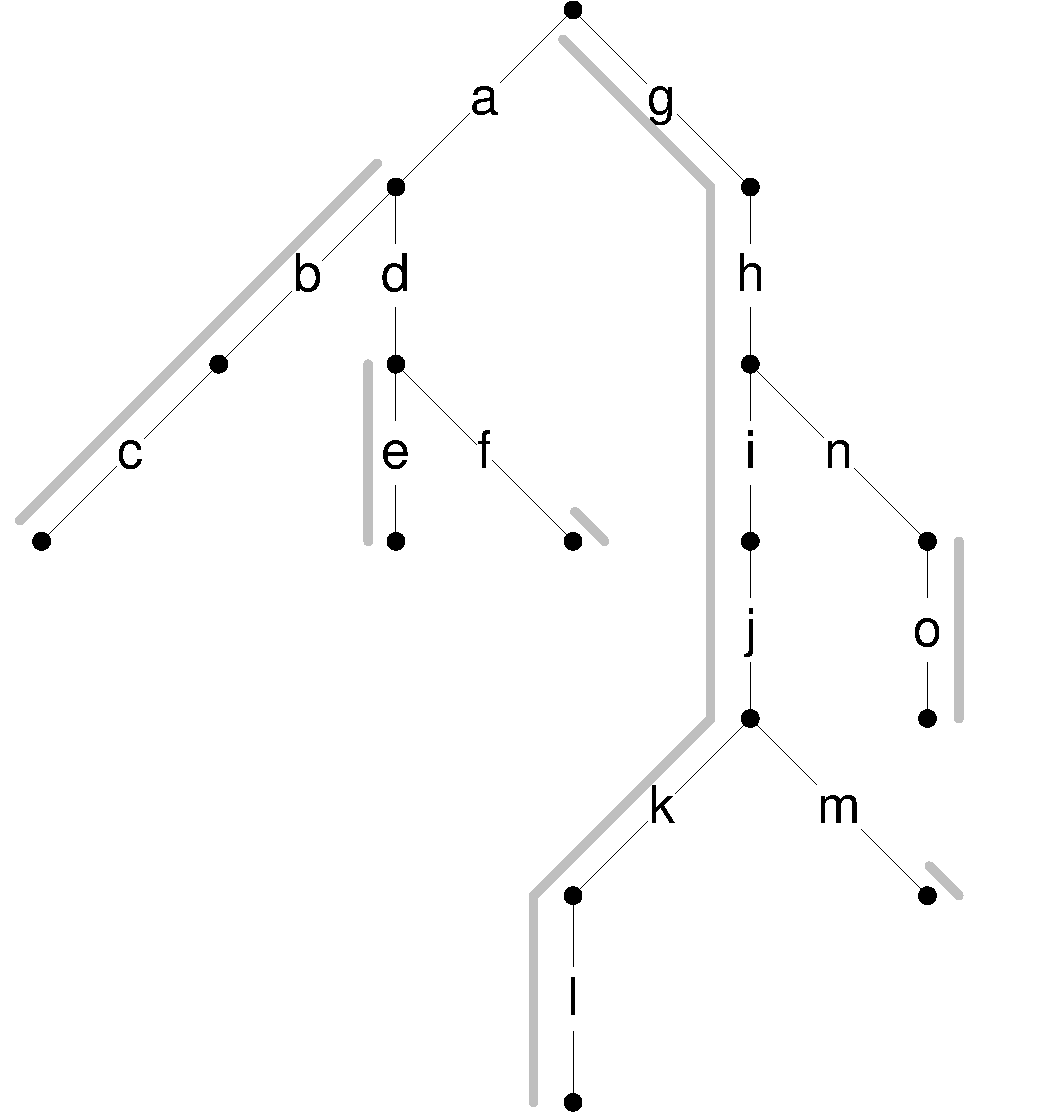
\includegraphics[width=0.4\textwidth,page=1]{ladder.pdf}
        \includegraphics[width=0.4\textwidth,page=2]{ladder.pdf}
    \end{center}
    \caption{\label{fig:ladder-ds} Ladders of a tree before and after their length is doubled. A \proc{LadderLce} string $s$ for this ladder decomposition is $s=abc|ade|f|ghijkl|hno|m$, where the splits between ladders are marked with a vertical line.}
\end{figure}

The \proc{LadderLce} data structure consists of the following:
\begin{itemize}
\item An input tree $T$ with a ladder decomposition.
\item A strings $s$, which is a concatenation of ladder labels for each ladder in $T$, where a ladder label is the concatenation of labels of edges between nodes in the ladder. \pref{fig:ladder-ds} shows an example of $s$.
\item For a node $u$, $\textit{index}(u)$ is an index in $s$ within the ladder label of $u$'s ladder, where $\zlabel(u)$ is stored.
\item Data structures for constant time LA on $T$ and constant time LCE on $s$.
\end{itemize}

\begin{lemma}
The \proc{LadderLce} data structure takes $O(n)$ space.
\end{lemma}
\begin{proof}
The string $s$ contains at most $2n$ characters. The rest of the data structures takes $O(n)$ space.
\end{proof}

\begin{lemma}
We can preprocess the \proc{LadderLce} data structure in $O(\sortt)$ time.
\end{lemma}
\begin{proof}
Constructing $s$ from the ladders takes $O(n)$ time, and preprocessing it for constant time LCE takes $O(\sortt)$ time. The rest of the data structures have $O(n)$ preprocessing times.
\end{proof}

\subsubsection{Query}

The \proc{LadderLce} query starts with $v=0$ and repeats the following:
\begin{enumerate}
\item Stop when $d_i(v) = w_i$ or $d_j(v) = w_j$ and return $v$.
\item Find $m_i = d(v_i')-d(p_i(v))$ and $i = \textit{index}(v_i') - m_i + 1$, where $v_i'$ is the node half way from $p_i(v)$ to $w_i$.
\item Find $m_j = d(v_j')-d(p_j(v))$ and $j = \textit{index}(v_j') - m_j + 1$, where $v_j'$ is the node half way from $p_j(v)$ to $w_j$.
\item Find $v' = LCE_s(i,j)$
\item Stop if $v' < \min(m_i,m_j)$ and return $v+v'$.
\item Otherwise add $\min(m_i,m_j)$ to $v$.
\end{enumerate}

\begin{lemma}
The \proc{LadderLce} query finds the correct LCE value.
\end{lemma}
\begin{proof}
The algorithm maintains the invariant that $v\leq\LCE(p_i,p_j)$. Which means that we know that $\zlabel(p_i(v))=\zlabel(p_j(v))$, but we do not know if $\zlabel(p_i(v+1))=\zlabel(p_j(v+1))$.

In step two, $i$ refers to a position in $v_i'$'s ladder, because the height of $v_i'$ is at least $m_i$. Therefore $s[i\twodots i+m_i-1]$ is the label of the path from $p_i(v)$ to $v_i'$, and similarly $s[j\twodots m_i-1]$ is the label of the path from $p_j(v)$ to $v_j'$. The LCE query thus determines the LCE value starting from $p_i(v+1)$ and $p_j(v+1)$ until we reach either $v_i'$ or $v_j'$, whichever comes first, which is distance $\min(m_i,m_j)$ from $d_i(v)$ and $d_j(v)$. When $v' < \min(m_i,m_j)$, we have found the final LCE value within the current pair of ladders and we can stop, otherwise we need to continue looking at other ladders.
\end{proof}

\begin{lemma}
The \proc{LadderLce} query takes $O(\log n)$ time.
\end{lemma}
\begin{proof}
Each iteration is constant time, and in each iteration we halve the distance between $d_i(v)$ and $w_i$ or between $d_j(v)$ and $w_j$.
\end{proof}

\proc{LadderLce} is very similar to \proc{HeavyPathLce}, however it has an extra property, which \proc{HeavyPathLce} does not have: If $\LCE(p_i,p_j)$ is less than half the length of $p_i$ and less than half the length of $p_j$, the LCE query takes constant time, since it only needs to look at one ladder.


\fi % report

%%%%%%%%%%%%%%%%%%%%%%%%%%%%%%%%%%%%%%%%%%%%%%%%%%%%%%%%%%%%%%%%%%%%%%%%%%%%%%%
%%%%%%%%%%%%%%%%%%%%%%%%%%%%%%%%%%%%%%%%%%%%%%%%%%%%%%%%%%%%%%%%%%%%%%%%%%%%%%%
\begin{thebibliography}{9}

\bibitem{ilie-navarro-tinta} Lucian Ilie, Gonzalo Navarro, and Liviu Tinta. The longest common extension problem revisited and applications to approximate string searching. Journal of Discrete Algorithms, Volume 8, Issue 4, December 2010, pages 418-428.

% \bibitem{linear-lcp} Toru Kasai, Gunho Lee, Hiroki Arimura, Setsuo Arikawa, and Kunsoo Park. Linear-Time Longest-Common-Prefix Computation in Suffix Arrays and Its Applications. CPM 2001, LNCS 2089, 2001, pages 181-192.

\bibitem{sort-complexity} Martin Farach-Colton, Paolo Ferragina, and S. Muthukrishnan. On the sorting-complexity of suffix tree construction. J. ACM Vol. 47, No. 6, November 2000, pages 987-1011.

\bibitem{karp-miller-rosenberg} Richard M. Karp, Raymond E. Miller, and Arnold L. Rosenberg. 1972. Rapid identification of repeated patterns in strings, trees and arrays. In Proceedings of the fourth annual ACM symposium on Theory of computing (STOC '72). ACM, New York, NY, USA, 125-136.

\bibitem{nca} D. Harel, R. E. Tarjan. Fast Algorithms for Finding Nearest Common Ancestors. SIAM J. Comput., 1984.
% S. Alstrup, C. Gavoille, H. Kaplan, and T. Rauhe. Nearest Common Ancestors: A Survey and a New Algorithm for a Distributed Environment. Theory of Comput. Sys., 2004.

\bibitem{jf-rmq} Johannes Fischer, and Volker Heun. Theoretical and Practical Improvements on the RMQ-Problem, with Applications to LCA and LCE. Proceedings of the 17th Annual Symposium on Combinatorial Pattern Matching (CPM'06), Lecture Notes in Computer Science 4009, 36-48, Springer-Verlag, 2006.

\bibitem{predecessor} Dan E. Willard. Log-logarithmic worst-case range queries are possible in space $\Theta$(N). Information Processing Letters, Volume 17, Issue 2, 24 August 1983, pages 81-84.

\bibitem{level-ancestor} Michael A. Bendera, Martín Farach-Colton. The Level Ancestor Problem simplified. Theoretical Computer Science 321, 2004, pages 5-12.

\bibitem{approx-search} Gad M. Landau and Uzi Vishkin. Introducing efficient parallelism into approximate string matching and a new serial algorithm. 18th ACM STOC, pages 220–230, 1986.

\end{thebibliography}

\ifreport

%%%%%%%%%%%%%%%%%%%%%%%%%%%%%%%%%%%%%%%%%%%%%%%%%%%%%%%%%%%%%%%%%%%%%%%%%%%%%%%
%%%%%%%%%%%%%%%%%%%%%%%%%%%%%%%%%%%%%%%%%%%%%%%%%%%%%%%%%%%%%%%%%%%%%%%%%%%%%%%
\section*{THE END}

\begin{comment}
\subsection*{Tinta tests}
The two tests of LCE query performance used in the Tinta paper are shown in \pref{alg:tinta-testlceonebyone} and \pref{alg:tinta-randomtestlce}.

% http://www.cs.dartmouth.edu/~thc/clrscode/clrscode.sty

\begin{algorithm}
\caption{Test algorithm for \texttt{test\_lce\_one\_by\_one}\label{alg:tinta-testlceonebyone}}
\begin{codebox}
\li \For each $LCE \in Algorithms$
    \Indentmore
\li     \For $k = 2$ \To $n$
        \Indentmore
\li         $A =\{(i,j) ~|~ j-i=k\}$
\li         \Repeat 3 times
\li             shuffle $A$
\li             start timing
\li             \For each $(i,j) \in A$
                \Indentmore
\li                 $LCE(i,j)$
                \End
\li             end timing
            \End
\li         $avg =$ average of the 3 timings
\li         log(each of the 3 timings)
\li         print($avg/length(A)$)
        \End
    \End
\end{codebox}
\end{algorithm}

\begin{algorithm}
\caption{Test algorithm for \texttt{random\_test\_lce}\label{alg:tinta-randomtestlce}}
\begin{codebox}
\li \Repeat 3 times
\li     $A =$ generate 1000000 random pairs $(i,j)$ where $i<j$
\li     \For each $\proc{LCE} \in \id{Algorithms}$
        \Indentmore
\li         start timing
\li         \For each $(i,j) \in A$
            \Indentmore
\li             $LCE(i,j)$
            \End
\li         end timing
        \End
    \End
\li \For each $LCE \in Algorithms$
    \Indentmore
\li     log(each of the 3 timings)
    \End
\li \For each $LCE \in Algorithms$
    \Indentmore
\li     print($($ average of the 3 timings $)/length(A)$)
    \End
\end{codebox}
\end{algorithm}
\end{comment}

\ifarticle
\fxfatal{Opskriv funktioner for plads.}
\fi % article

\subsection*{Dropped}
\begin{enumerate}
\item DOC: Test on another machine.
\item CODE: Improve cache-vertical and make shift variant.
\item CODE: Non-random strings? Non-random queries? Different t-values for Hash-3L?
\end{enumerate}

\listoffixmes

\begin{comment}
\section{What is the time for KMR?}
\subsection{Original KMR}
"Rapid identification of repeated patterns in strings, trees and arrays"
says $O(n\cdot(\log n)^2)$.

http://portal.acm.org.globalproxy.cvt.dk/citation.cfm?id=804905

\subsection{RMR in $O(n \log n)$}
\begin{itemize}
\item
"A Theoretical and Experimental Study on the Construction of Suffix Arrays in External Memory"
page 10, 3.3 The Doubling Algorithm.

http://www.springerlink.com.globalproxy.cvt.dk/content/h1tejj3bamjj5qrg/
\item
"Compressing and indexing labeled trees, with applications"

http://portal.acm.org.globalproxy.cvt.dk/citation.cfm?id=1613680
\end{itemize}

KMR uses $O(sort(n,n^2)\cdot\log n) = O(n\log n)$ time.

At a given level:
\begin{enumerate}
\item create 2-touples of fingerprints from the previous level.
\item sort these touples lexicographically. (radix sort takes $O(kn)$ for $\sigma=n^k$, here $\sigma=n^2$)
\item scan through the sorted touples to assign new fingerprints.
\end{enumerate}
\end{comment}

\fi % report

\end{document}
